
% \section{Introduction}
% \label{sec:introduction-rsgm}
\emphmarginnote{Score-based Generative Models} (SGMs) also called diffusion models \parencite{song2019generative,song2020score,ho2020denoising,nichol2021beatgans} formulate generative modelling as a denoising process.
Noise is incrementally added to data using a diffusion process until it becomes approximately Gaussian.
The generative model is then obtained by simulating an approximation of the corresponding time-reversal process, which progressively denoises a Gaussian sample to obtain a data sample.
This process is also a diffusion whose drift depends on the logarithmic gradients of the noised data densities, i.e. the Stein scores, estimated using a neural network via score matching \parencite{hyvarinen05a,vincent2011connection}.

SGMs have been primarily applied to data living on Euclidean spaces, i.e. manifolds with flat geometry.
However, in a large number of scientific domains the distributions of interest are supported on Riemannian manifolds.
These include, to name a few, protein modelling \parencite{shapovalov2011smoothed}, cell development \parencite{klimovskaia2020poincare}, image recognition \parencite{lui2012advances}, geological sciences \parencite{karpatne2018machine,peel2001fitting}, graph-structured and hierarchical data \parencite{roy2007learning,steyvers2005large}, robotics \parencite{feiten2013rigid,senanayake2018directional} and high-energy physics \parencite{brehmer2020flows}.

In this chapter we develop \emphmarginnote{Riemannian Score-based Generative Models}, an extension of score-based generative models to Riemannian manifolds.
The objective is to incorporate the geometry of the problem at hand by respecting the natural setting of the data being modelled.
This requires constructing a noising process on the manifold that converges to an easy-to-sample reference distribution.
We establish that, as in the Euclidean case, the corresponding time-reversal process is also a diffusion whose drift includes the Stein score which is intractable but can similarly be estimated via score matching.
Methodological extensions are required as in most cases the transition kernel of the noising process cannot be sampled exactly.
For example on compact manifolds it is typically only available as an infinite sum through the Sturm--Liouville decomposition \parencite{chavel1984eigenvalues}.
To this end, we develop non-standard techniques for score estimation and rely on the use of Geodesic Random Walks for sampling \parencite{jorgensen1975central}.
We provide theoretical convergence bounds for RSGMs on compact manifolds and demonstrate our approach on a range of manifolds and tasks, including modelling a number of natural disaster occurrence datasets collected by \textcite{mathieu2020riemannian}.
We show that RGSMs achieve better performance than recent baselines \parencite{mathieu2020riemannian,rozen2021moser} and scale better to

\section{Euclidean Score-Based Generative Modelling}

Having introduced many tools in the background material, we can now see how these come together to produce the class of models known as "diffusion models" or "score-based generative models".
Both of these terms capture part of the type of model that they are applied to, but neither is fully descriptive.
There are two perspectives on diffusion models; discrete-time diffusion models \parencite{sohl2015deep,ho2020denoising} and continuous-time diffusion models \parencite{song2020score}.
These are related, and the discrete-time models can be seen as a discretisation of the continuous-time.
As such, this presentation will focus only on the continuous-time version, but will highlight where the discrete approximation comes into play.
Throughout we will work with a state space of dimension \(d\), such that a data point is an element \(\v{X}\in \R^d\).

Diffusion models are strongly related to other classes of deep generative models.
They follow a common paradigm of taking simple to sample noise, typically a multi-dimension Gaussian random variable, and through a series of transformations try to turn this into the distribution of interest.
Most similar are normalising flows, which also fit into the described category.
We shall see later that there are deep connections between diffusion models and continuous normalsing flows.

Let us briefly describe the process for constructing a diffusion model.

We start with a density \(\pi\) that we wish to learn to sample from.
Let us assume that we either have a set of samples and cannot access more, or that it is expensive to do so, and that we have no access to the likelihood or an unnormalised version of this.
Our goal is to have a model from which we can sample, and compute the likelihood for samples from for the distribution \(\pi\).

A summary of the diffusion modelling strategy is:
\1 First we will evolve this density under a stochastic differential equation, which we shall term the forward or noising SDE.
We will from now denote this SDE as \(\del{\Xf_t}_{t\in\sbr{0, T}}\), denoting the forward direction.
These SDEs have an equation of the form \[\d \Xf_t= \v{b}(\Xf_t, t) \d t + \v{\sigma}(\Xf_t, t) \d \v{B}_t\] ref to earlier.
We shall require that this SDE is that at "large" times converges to a distribution for which we know the density and can sample from.
We will evolve this SDE up to a chosen time \(T\) which is large enough for such convergence to occur.
Let us denote the desity of this SDE at time \(t\) as \(\pi_t\).
\2 Using a time reversal result, we can obtain a stochastic differential equation that has the same sample paths as our forward noising SDE, but with time in the reverse direction.
We shall term this the reverse or denoising SDE, and we will start it from time \(T\) in the forward SDE from the distribution of \(\Xf_T\) and run it backwards.
We will denote this reverse SDE as \(\del{\Xb_t}_{t\in\sbr{0, T}}\) to emphasise it is an SDE with the same paths, but with time running in the other direction.
We will use the convention that time in the reverse SDE is opposite to that of the forward SDE, i.e. that \(\Xf_t = \Xb_{T-t}\).
While this makes it necessary to track if one is talking about the forward or backward SDE to determine when a given time refers to, it means one does not have to deal with Brownian motions going backward in time, which can be more confusing.
This reverse SDE then has the equation \[\d \Xb_t = \sbr{-\v{b}(\Xb_t, t) + \nabla_{\Xb_t} \log \pi_{T-t}(\Xb_t) }\d t + + \v{\sigma}(\Xb_t, t) \d \v{B}_t\].
Note the time reindexing of time in the term \(\pi_{T-t}\) as the density of the reverse SDE at time \(t\) is the same as the density of the forward SDE at time \(T-t\).
\3 All the terms in the reverse SDE are known, except for the "score" term, \(\nabla_{\Xb_t} \log \pi_{T-t}(\Xb_t)\).
We therefore need a method to approximate or learn this term.
Fortunately, with the large score matching toolbox we have available to us there are several options for learning this score.
\4 Using the standard toolkit of SDE sampling schemes we can sample the reverse SDE in practise.
\5 Using the connection between an SDE and the associated ODE we can evaluate the likelihood of a sample under the model, using standard ODE solving toolkits.
\0

Let us in detail look at each of these steps. 

\subsubsection{The forward noising SDE}

The first stage of a diffusion model is to corrupt the data towards a known and tractable noise distribution, often referred to as the "reference distribution".
The point of this step is to define a path between the distribution of interest and an easy to sample distribution, with the intent later on of following this path in the reverse direction.
Let us denote the reference distribution as \(\pi_T\), to suggest it is the distribution the forward SDE will arrive at some large time \(T\).
If we make our choices right, this will be true up to a small error.

Recall that if we have access to a density of the form \(\pi(x) \propto \exp(-U(x))\), then the SDE \[\d \v{X}_t = \nabla_{\v{X}} U(\v{X}) \d t + \sqrt{2} \d \v{B}_t\], will in the limit of infinite time converge to \(\pi\), regardless of the distribution we initialise the SDE with.
% \todo{say something about convergence rate?} 
We can also rescale this SDE by a time dependant noise factor, \(\beta({t})\), and obtain the same result, giving an SDE of the form \[\d \v{X}_t = \beta(t) \nabla_{\v{X}} U(\v{X}) \d t + \sqrt{2 \beta(t)} \d \v{B}_t\].
This time rescaling can be very useful in diffusion models in optimising the efficiency of the discretised model rollouts and focusing the majority of the learning power of the score network on important regions of the SDE.
% \todo{decide if to suppress notation or not.}

While using Langevin dynamics to sample from complex distribution can be very slow to mix effectively, sampling a simple unimodel distribution is very fast.
This gives us an option for our SDE that converges for a known distribution.
Choosing the unit Gaussian as our reference distribution, \(\pi_T(\v{X}) \propto \exp\del{-\tfrac{1}{2} \v{X}^T \v{X}}\), we arrive at \(U(\v{X}) = -\v{X}\), and thus a forward noising SDE of the form \[\d \Xf_t = -\Xf_t\d t + \sqrt{2} \d \v{B}_t \].
This is the well known Ornstein–Uhlenbeck process, and this converges exponentially quickly towards the unit Gaussian.
This is an ideal noising SDE given the exponential convergence and the tractability of the density and of sampling of the Gaussian reference distribution.
In the literature this is typically known as the "variance preserving SDE" or "VP-SDE".
A property that will be useful later is that the transition density in the forward direction, \(p_{s|t}\delvert{\Xf_s}{\Xf_t}, \; s > t\) has analytic density and sampling.
For an SDE with noising schedule \(\beta(t)\) this is given by \[ p_{s|t}\delvert{\v{X}_s}{\v{X}_t} = \c{N}\delvert{\v{X}_s}{e^{-{\int_t^s \beta(\tau)\d\tau}} \v{X}_t, \del{1-e^{-2{\int_t^s \beta(\tau)\d\tau}}}\v{I}}\]

The other common alternative is the "variance exploding SDE" or "VE-SDE".
In this we simply apply Brownian motion as the noising SDE.
This will not converge to a stable distribution.
However, the transition density of this SDE is given by \[\textstyle p_{s|t}\delvert{\Xf_s}{\Xf_t} = \c{N}\delvert{\Xf_s}{\Xf_t, \sqrt{{\int_t^s} \beta(\tau)\d\tau}\v{I}}\].
The variance of this will continue to grow with time and eventually the variance of this transition density will dominate the variance of \(\pi\), and so the distribution \[\pi_T(\Xf_t) = \int p_{T|0}\delvert{\Xf_T}{\Xf_0} \pi(\Xf_0) \d \Xf_0\] will be well approximated by \(\c{N}\delvert{\Xf_T}{\v{0}, \sqrt{{\int_t^s} \beta(\tau)\d\tau}\v{I}}\), and therefore we can use this as the reference distribution.

An alternative way to choose the forward stochastic differential eqaution is to start with the forward transition density and work backwards to the coeficients. If we restrict ourselves to linear Guassian transition densities, those of the form 
\[p_{t|0}(x_t | x_0) = \c{N}(x_t; \alpha_t x_0, \sigma^2_t)\]
for some differentiable mean function \(\alpha_t:\R\to \R\), with the restriction that \(\alpha_0=1\), and differentiable noise function \(\sigma_t:\R\to\R\), with the restriction that \(\sigma_0=0\), then the stochastic differential equation that has this forward transition density is
\[\d\v{X}_t = \od{\log \alpha_t}{t}\d t +  \sbr{\od{\sigma_t^2}{t} - \od{\log \alpha_t}{t} \sigma_t^2}\d\m{B}_t\]
If we pick \(\alpha_t\) and \(\sigma_t\) such that as \(t\to T\), \(\alpha_t\to 0\), then the process will converge to the distribution \(\c{N}(x_T; 0, \sigma_T^2)\), giving us a reference distribution to work with.

The VP-SDE and VE-SDE can be fit into this framework, with \[&\alpha_t =  \exp(-\int_0^t \beta(\tau) \d\tau)\quad &\sigma_t &= 1- \exp(-2\int_0^t \beta(\tau) \d\tau)\quad&\text{VP-SDE}\\
&\alpha_t =  1\quad &\sigma_t = \int_0^t \beta(\tau) \d\tau\quad&\text{VE-SDE}\]



The choice of forward noising stochastic differential equation can have a significant impact on performance of a diffusion model. Interesting empirical studies can be seen for example in \textcite{karras2022Elucidating}.

\begin{table}[h]
	\centering
	\begin{tabular}{lcccr}
		\toprule
		{\scshape SDE}                              &  & & {\scshape Complexity} & {\scshape Variance} \\
		& \makecell{Samples from \(p_{t|s}\)} & \makecell{Analytic \(\nabla \log p_{t|s}\)} & & \\
		\midrule
		{\(\ssmlosst{}\)}  & \cmark & \xmark & \(\c{O}(d)\) & Highest\\
		{\(\ismlosst{}\)}  & \cmark & \xmark & \(\c{O}(d^2)\) & Middle\\
		{\(\dsmlosst{}\)}  & \cmark & \(t-s\) small & \(\c{O}(d)\) & Lowest \\
		{\(\gdsmlosst{}\)} & \cmark & \cmark & \(\c{O}(d)\) & Lowest \\
		\bottomrule
	\end{tabular}
	\caption{A comparison of score-matching objectives for diffusion models}
	\label{tab:loass_comparison}
\end{table}

% Typically in generate models such as VAEs and normalising flows the transformation we ask the model a model to turn random noise in to interesting data through a series of intermediate steps. The intermediate steps, and the path on should take between each of these however remain unspecified, and the model must learn to pick one possible solution from a typically infinite set of choices. By contrast \emphmarginnote{diffusion models} specify the whole generative process process from the simple noise distribution to the data distribution. This specification of the mapping is a key element in their success. It significantly reduces the task we ask the model to learn from that of exploring the infinite space of possible mappings between data and noise, to a simple regression problem of matching the pre-specific path. The innovation in these models is being able to specify this mapping, and train the resulting model in an efficient way.

% In the following I consider the continuous time formulation of diffusion models introduced in \textcite{song2020score}, which defines the corruption of noise into data via an SDE. There also exists the discrete view of diffusion modelling \textcite{sohl2015deep,ho2020denoising} where the corruption of data is done in a series of discrete step. Since the links between the two are very clear, and the discrete view can be seen as a discretisation of the continuous time version, I will not develop this.

% The recipe for producing a diffusion model has two key steps:
% \1 Specify a way of corrupting data into noise via a diffusion equations.
% \2 Reverse this process of corruption to be able to turn noise into data, giving us a generative model. 
% \0
% This recipe as it turns out can be applied much more general than diffusion models, and this will be discussed later, but for now we will consider the case of modelling distributions supported on \(\R^n\) using diffusions as the corrupting process.

% The main tool for this corruption is a \emphmarginnote{stochastic differential equation} (SDE). Typically we use \emphmarginnote{linear SDEs}. These have the form \[\d \v{X}_t = b(\v{X}_t, t) \d t + \Sigma(\v{X}_t, t) \d \v{B}_t\] where \(b : \R^n \times \R \to \R^n\) and \(\Sigma : \R^n \times \R \to \R^{(n\times n)}\).

\subsubsection{Applying a time reversal result}

The crucial step to be able to follow backwards the path defined by our forward noising SDE is the application of a time reversal result.
We have discussed these theoretically earlier in \cref{sec:time-reversal} but to briefly recap;

For a forward-time stochastic differential equation 
\[ \d\Xf_t = \v{b}(\Xf_t, t)\d t + \sigma(t)\d \Bf_t, \quad \Xf_0 \sim p_0\]
with time-marginal distributions \(p_t(\v{X})\), the reverse-time stochastic differential equation
\[\d\Xb_t = \sbr{\v{b}(\Xb_t, t) - \sigma(t)^2\nabla\log p_t(\Xb_t)}\d t + \sigma(t)\d \Bb_t, \quad \Xb_T \sim p_T\].
has the same time-marginal distributions \(p_t(\v{X})\) as the forward-time stochastic differential equation.

\subsubsection{Learning the score}

The next step in producing a diffusion model is learning the score term that appears in the reverse SDE, \(\nabla_{\v{X}_t} \log p_t(\v{X}_t)\).
At first glance this may seem difficult, but a strong literature exists on learning this term, known as \emphmarginnote{score matching}.
In order to approximate this score function, we will use an approximation taking inputs \(\v{X}_t\) and \(t\).
We will denote this \(\scorenet{}: \R^d \times \sbr{0, T} \to \R^d\).
We will also use the notion \(\scorenett{} : \R^d \to \R^d\) to refer to this function partially evaluated at time \(t\), \(\scorenett{}(\cdot) = \scorenet(\cdot, t)\).
Typically, we will make this a neural network of some kind, and look to optimise this via gradient-based learning.

% \emphmarginnote{Implicit score matching (ISM)} \parencite{hyvarinen05a} says that the following is true for a density \(\pi\) supported on \(\R^d\) relative to the Lebesgue measure;
% \[\nabla_{\v{X}} \log \pi(\v{X}) = \argmin_{\phi} \int_{\R^d} \cbr{ \frac{1}{2} \norm{\phi\del{\v{X}}}^2 + \dive(\phi)(\v{X})} \pi(\v{X}) \d \v{X} \].
% We can apply this to our SDE setting to say that the score at a given time is given by \[\nabla_{\v{X}} \log \pi_t(\v{X}) = \argmin_{\scorenett{}} \int_{\R^d} \cbr{ \frac{1}{2} \norm{\scorenett{}(\v{X})}^2 + \dive(\scorenett{})(\v{X})} \pi_t(\v{X}) \d \v{X}\].
% We denote then this loss function as \(\ismlosst{}: \scorenett \mapsto \R\) such that \(\nabla_{\v{X}} \log \pi_t(\v{X}) = \argmin_{\scorenett{}} \ismlosst{}\).
\textcite{hyvarinen05a} proves the following result
\begin{theorem}[Implicit score matching (ISM)]
	\label{def:ism}
	Consider a density \(p_a(A)\) supported on \(\R^d\) relative to the Lebesgue measure.
	Then,
	\[\nabla_{A} \log p_a(A) = \argmin_{g\text{ measurable in }L^2} \E_{A}\sbr{ { \tfrac{1}{2} \norm{g\del{A}}^2 + \dive(g)(A)}}.\]
\end{theorem}
Using this we can learn the score of a distribution \(p_a\) if we just have access to good samples from \(p_a\) as we can approximate this expectation with Monte Carlo estimation.

We can apply this to our SDE setting to say that the score at a given time is given by \[\nabla_{\v{X}_t} \log p_t(\v{X}_t) = \argmin_{\scorenett{}} \E_{\v{X}_t} \sbr{ \tfrac{1}{2} \norm{\scorenett{}(\v{X}_t)}^2 + \dive(\scorenett{})(\v{X}_t)}\].
We denote then this loss function as \(\ismlosst{}\).

In order to draw samples from \(p_t(\v{X}_t)\) we can utilise the fact that \[p_t(\v{X}_t) = \int p_{t|0}(\v{X}_t) p_0(\v{X}_0) \d \v{X}_0\].
We can sample then from this joint density as we have as our dataset samples from \(p_0 = \pi\), and we have access to sampling from the transition density \( p_{t|0}\) from the forward noising SDE.
We then throw away the samples from \(p_0\) to obtain samples from \(p_t\).

What is not so nice about this objective is that it requires computation of the divergence of the score.
While this is achievable using automatic differentiation packages, it is expensive in high dimension, scaling in cost with \(\c{O}(d^2)\).

It is possible to apply to this the Hutchinson trace trick estimator \parencite{hutchinson1989stochastic} to stochastically approximate the divergence to get a loss function that scales with \(\c{O}(d)\) at the cost of higher variance, as detailed in \textcite{song2020sliced}, where it is called \emphmarginnote{sliced score matching (SSM)}.
We denote this loss function \(\ssmlosst{}\).
In practise this additional variance does not seem to be too important, as the variance of the Monte Carlo estimation of the integral over \(p_t\) is larger.

\emphmarginnote{Denoising score matching (DSM) \label{def:dsm}} \parencite{vincent2011connection} is an alternative approach to implicit score matching that typically has lower variance.
We do not get this for free, as we will need to know a little more information to apply this.
Recall that the definition of the conditional distribution states that for \(L^2\)-integrable random variables \(A\) and \(B\), \[\argmin_{g\text{ measurable in }L^2} \E_{A, B}\sbr{\norm{A - g(B)}^2} = g: b\mapsto\E_{A}\sbrvert{A}{B=b}\], where \(\E_{A}\sbrvert{A}{B=b}\) is the conditional expectation of \(A\) given a value of \(B\).
We apply this by putting \(A = \nabla \log p_{c|d}\delvert{C}{D}\) and \(B = C\) for new random variables \(C\) and \(D\), assuming they have densities relative to the Lebesgue measure, and so \[g(C) = \E_{D}\sbrvert{ \nabla \log p_{c|d}\delvert{D}{C}}{C}\].
We can then apply the Tweedie identity.
\begin{lemma}[The Tweedie identity]\label{lem:tweedie}
	\[\E_{D}\sbrvert{\nabla_{C} \log p_{c|d}\delvert{C}{D}}{C} = \nabla_{C} \log p_c(C)\]
\end{lemma}
\begin{proof}
	Delayed to \cref{sec:tweedie_proof}
\end{proof}
Combing this we see that \[ \argmin_{g\text{ measurable in }L^2} \E_{C,D}\sbr{\norm{\nabla_C \log p_{c|d}\delvert{C}{D} - g(C)}^2} &= \E_{D}\sbrvert{\nabla_{C} \log p_{c|d}\delvert{C}{D}}{C}\nonumber \\ &= \nabla_{C} \log p_c(C)\], and therefore can learn the score for \(\nabla_C \log p_c(C)\) if we have access to \1 samples from the joint distribution \(p_{c,d}(C, D)\) and \2 access to the analytic conditional score \(\nabla_C \log p_{c|d} \delvert{C}{D}\).\0

To apply this to our SDE setting, we pick \(C = \v{X}_t\) and \(D=\v{X}_s\), with \(s < t\). We have access to samples from \(p_{t,s}\del{\v{X}_t, \v{X}_s}\) by using the fact that 
\[
	p_{t,s}\del{\v{X}_t, \v{X}_s} &= \int_{\R^d} p_{t|s, 0}\delvert{\v{X}_t}{\v{X}_s, \v{X}_0} p_{s|0} \delvert{\v{X}_s}{\v{X}_0} p_0\del{\v{X}_0} \d \v{X}_0 \\
	&= \int_{\R^d} p_{t|s}\delvert{\v{X}_t}{\v{X}_s} p_{s|0} \delvert{\v{X}_s}{\v{X}_0} p_0\del{\v{X}_0} \d \v{X}_0
\] where the second line follows as SDE transitions have the Markov property. We have access to samples from \(p_0\) from our data, and the SDE tells us how to sample from the transitions.
We also need access to the analytic form of \(\nabla_{\v{X}_t} \log p_{t|s} \delvert{\v{X}_t}{\v{X}_s}\).
For most SDEs used in the literature, such as the variance exploding and preserving, this is available.
If it is not available, often good approximations are available over for short time steps between \(s\) and \(t\).

The most common form of this loss in the literature is to set \(s=0\). 
This simplifies the sampling as then we only need to sample the one transition.
This is the denoising score matching described in \textcite{song2020score}.
We describe the more general scheme here as it is useful when we only have access to an approximation of \(p_{t|s}\) over short times.

We shall label this loss \(\gdsmlosst{}\) in the general case and \(\dsmlosst{}\) when using \(s=0\).

To summarise:
\begin{table}[h]
	\centering
	\begin{tabular}{lcccr}
		\toprule
		{\scshape Loss}                              & \multicolumn{2}{c}{{\scshape Requires}} & {\scshape Complexity} & {\scshape Variance} \\
		& \makecell{Samples from \(p_{t|s}\)} & \makecell{Analytic \(\nabla \log p_{t|s}\)} & & \\
		\midrule
		{\(\ssmlosst{}\)}  & \cmark & \xmark & \(\c{O}(d)\) & Highest\\
		{\(\ismlosst{}\)}  & \cmark & \xmark & \(\c{O}(d^2)\) & Middle\\
		{\(\gdsmlosst{}\)}  & \cmark & \(t-s\) small & \(\c{O}(d)\) & Lowest \\
		{\(\dsmlosst{}\)} & \cmark & \cmark & \(\c{O}(d)\) & Lowest \\
		\bottomrule
	\end{tabular}
	\caption{A comparison of score-matching objectives for diffusion models}
	\label{tab:loass_comparison}
\end{table}

The objectives detailed match the score at given time \(t\) only. 
In order to match the score at all times, we integrate this objective over all times \(t \in \sbr{0, T}\).
\[\ell(\scorenet{}) = \int_{\sbr{0, T}} \lambda(t) \ell_t(\scorenett{}) \d t\].
Notice there is a weighting function applied over all \(t\).
While this weighting does not affect the minima of the objective, it does rebalance where a network will prioritise learning the score most.
Many choices for \(\lambda(t)\) exist and can be tuned to optimise different objectives.
In particular picking \(\lambda(t) = \sigma(t)^2\) can be shown to be equivalent to optimising the maximum likelihood objection on the dataset \cite{huang2021variational,durkan2021maximum}.

A common feature of all of these objectives is that they are
\1 stable regression objectives and
\2 require evaluation of the score network at a given time \(t\) only.
\0
Compare this to the objectives of normalsing flow models, VAE models, or GANs.
These objective functions require us to run a full generation of samples from the model in order to evaluate the objective.
In contrast, the score matching objectives only need us to evaluate the generative model at one point in the generative process.
Additionally, the score matching objectives at a given time is stable with respect to other times.
The minima at a given time will not change as we optimise the score function at other times.
This is in comparison to other objectives where changing the weights at one point in the network significantly changes what the optimum weight at other points in the network is.
This is exacerbated in GANs, as changing the discriminator function changes the objective the generator function is trying to learn, leading to well known instabilities.
This cheap evaluation and objective stability is one of the key attractions of diffusion models.
It is akin to us being able to optimise the weights in each layer of one of these other types of model independently, and this optimisation not affect the optimal weights in other layers.

There is one common draw back to these objectives however, and that is the Monte Carlo sampling required to evaluate these objectives makes them particularly noisy as objectives.
This can be mitigated however by taking an average of the weights through training.
Typically, exponential moving averages have been used, and the smoothing rate requires tuning.
Recently, \textcite{karras2023analyzing} proposed new averaging schemes, and importantly a mehtod to perform hyperparameter optimisation of the smoothing rates post-hoc, requiring only a single training run of the model.

\subsubsection{Approximate sampling from SDEs}
\label{sec:sde_discretisation}

Much the computational impossiblity of solving genreal ODE problems exactly, it is impossible to sample from general SDEs exactly.
We can however make good approximations to this.

\subsubsection{Likelihood ODEs}
\label{sec:likelihood-ode}
The final thing that we are missing now is the ability to compute the likelihood of a sample from a diffusion model.
In order to do this we will leverage the \emphmarginnote{Fokker-Plank equation} (\cref{sec:fokker_plank}).
Recall that for an SDE of the form \[\d \v{X}_t = \v{b}(\v{X}_t, t) \d t + \m{\Sigma}(\v{X}_t, t) \d \v{B}_t \], in this case where \(\m{\Sigma}\) is a matrix of noise coefficients, the time-evolution of the density is given by
\[ \pd{p_t(\v{X})}{t} = -\sum_{i=1}^d \pd{}{\v{X}_i}\sbr{\v{b}(\v{X}, t) p_t{\v{X}}} + \frac{1}{2} \sum_{i=1}^d \sum_{j=1}^d \frac{\partial^2}{\partial \v{X}_i \partial \v{X}_j} \sbr{\m{\Sigma}(\v{X}, t) \m{\Sigma}(\v{X}, t)^T p_t(\v{X})} \].
Using this, we can obtain the following result

\begin{theorem}[The likelihood flow ODE]
	\label{thm:likelihood_ode}
	For an SDE of the form 
	\[\d \v{X}_t = \v{b}(\v{X}_t, t) \d t + \m{\Sigma}(\v{X}_t, t) \d \v{B}_t \]
	initialised with \(\v{X}_0 \sim p_0\), the ODE
	\[\d \v{X}_t = \sbr{\v{b}(\v{X}_t, t) - \frac{1}{2}\sbr{\nabla \cdot \sbr{\m{\Sigma}(\v{X}, t) \m{\Sigma}(\v{X}, t)^T}\nonumber +\m{\Sigma}(\v{X}, t) \m{\Sigma}(\v{X}, t)^T \nabla_{\v{X}_t}\log p_t(\v{X}_t)}} \d t\]
	initialised with \(\v{X}_0 \sim p_0\) has the same marginal density at all times \(t\in\sbr{0,T}\)
\end{theorem}
\begin{proof}
	Due to \textcite{maoutsa2020interacting} and \textcite[appendix D]{song2020score}, restated in \cref{sec:likelihood_ode_proof}.
\end{proof}
In diffusion models we typically use \(\m{\Sigma}(\v{X}, t) = \sigma(\v{X}, t) I\), a simple time-dependant scalar noise.
With this, the likelihood ODE simplifies to
\[\d \v{X}_t = \sbr{\v{b}(\v{X}_t, t) - \frac{1}{2}\sigma(\v{X}, t)^2 \log p_t(\v{X}_t)} \d t \label{eq:likelihood_ode_drift} \].
Fortunately there already exists tools to be able to compute the change in likelihood induced by an ODE trajectory, assuming the ODE describes the flow of a density.
\begin{theorem}[Instantanious change of likelihood of an ODE]
	Let \(\del{\v{X}_t}_{t\in\sbr{0,T}}\) be a stochastic process with marginal density at time \(t\) \(p_t(\v{X}_t)\).
	Let \(\d \v{X}_t = \v{b}(\v{X}_t, t) \d t\) be an ODE describing the evolution of particles.
	Assume that \(\v{b}\) is uniformly Lipshitz continuous in \(\v{X}_t\) and continuous in \(t\).

	Then, the instantaneous change in log probability is given by 
	\[\pd{\log p_t(\v{X}_t)}{t} = -\tr\del{\eval{\od{\v{b}}{\v{X}_t}}{\del{\v{X}_t, t}}} = \nabla \cdot \v{b}\del{\v{X}_t, t}\]
\end{theorem}
\begin{proof}
	Proved in \textcite[appendix A]{chen2018neural}. Restated in \cref{sec:ode_likelihood_formula}.
\end{proof}
Using this, we can evaluate the likelihood of a point under our diffusion model at \(t=0\).
For a given point \(v{X}_0\) is equal to the change in likelihood over the course of the ODE, plus the likelihood of the point at the other end, \[\log p_0(\v{X}_0) = \int_0^T \nabla \cdot \v{b}\del{\v{X}_t, t} \d t + \log p_T(\v{X}_T)\]
where \(\v{X}_t\) is the path the point \(\v{X}_0\) follows under the ODE.

In practise, we solve these as a joint ODE to take advantage of error tolerant solvers on the joint system,
\[
	\d 
	\begin{bmatrix}
		\v{X}_t \\ \log p(\v{X}_t)
	\end{bmatrix} = 
	\begin{bmatrix}
		\v{b}\del{\v{X}_t, t} \\ \nabla \cdot \v{b} \del{\v{X}_t, t}
	\end{bmatrix}
\]
This is in fact how \emphmarginnote{continuous noramlising flows (CNFs)} \parencite{chen2018neural} work. 
The model is defined by a parametrised drift function \(\v{b}_\theta\), and is trained by maximum likelihood by backpropogating through the ode solver \parencite{chen2018neural}. 
There exist a number of stratergies for backpropogating through ODE solvers.
These are discussed well in \textcite{kidger2021on}, which has accompanying it the python library \verb|diffrax| \marginnote{\url{https://github.com/patrick-kidger/diffrax}} for handling ODEs and other DEs easily.

To apply this scheme for computing the likelihood to diffusion models we simply use our modified drift function in \cref{eq:likelihood_ode_drift} and use the reference distribution from our diffusion model for \(p_T\).

This also gives us an additional method to sample from our diffusion model. 
Insdead of solving the SDE approximately (\cref{sec:sde_discretisation}) we can sample from \(p_T\) and solve this ODE in reverse to draw samples from the model.
This can outperform sampling the SDE in certain scenarios \parencite{karras2022Elucidating,song2019generative}.

\section{Riemannian Score-Based Generative Modelling}
\label{sec:score-appr-manif}
In the background material we introduced diffusion models defined over Euclidean space to model densities on \(\R^n\).
In this section, we introduce new tools and techniques to generalise diffusion models to Riemannian manifolds (without boundary).

More specifically our setting will be a \emphhyperref{complete}{def:complete_manifold}, \emphhyperref{orientable}{def:orientable_manifold}, \emphhyperref{connected}{def:connected_space}, \emphhyperref{boundaryless}{def:manifold_with_boundary} \emphhyperref{Riemannian}{def:riemannain_manifold} manifold, \((\c{M}, g)\).

Four components are required to extend SGMs to this setting: \begin{enumerate}[label=\roman*)] \item a forward {noising} process on \(\c{M}\) which converges to an easy-to-sample reference distribution, \item a time-reversal formula on \(\c{M}\) which defines a backward generative process, \item a method for approximating samples of SDEs on manifolds, \item a method to efficiently perform score matching on Riemannian manifolds.
\end{enumerate}
We provide these tools, and detail them now.

\subsection{Noising processes on manifolds}

\label{sec:non-compact}

The first necessary component is a suitable generic noising process on manifolds that will converge to a convenient stationary distribution.
In the background material we showed how the common noising processes used in Euclidean diffusion models are instances of \emphhyperref{Langevin dynamics}{sec:langevin_dynamics}. 
Recall these are given for an SDE in Euclidean space by
\[\d \v{X}_t = -\nabla_{\v{X}_t} U(\v{X}_t) \d t + \sqrt{2} \d\v{B}_t\]
and that this SDE will converge in distribution to a density, relative to the Lebesgue measure, proportional to \(\exp\del{-U\del{\v{X}_t}}\).
\todo[inline]{conditions on U?}

On Riemannian manifolds, we have very similar results for the equivalent Langevin stochastic differential equation.
\[ \d \v{X}_t = -\nabla_{\v{X}_t}^g U(\v{X}_t) \d t + \sqrt{2} \d\v{B}_t^M\]
where \(\nabla^g\) is the Riemannian gradient (see \cref{sec:riemannian_gradient}) and \(\d\v{B}_t^M\) is a Brownian motion associated with the manifold (see ...).
For example, it is easy to prove that a very similar stationary distribution exists
\begin{theorem}[Stationary distribution of Langevin dynamics on Riemannian manifolds]
	For a stochasitc differential equation of the form
	\[ \d \v{X}_t = -\nabla_{\v{X}_t}^g U(\v{X}_t) \d t + \sqrt{2} \d\v{B}_t^M\]
	the distribution \(\mu_U\) with Radon-Nikodyom derivate with respect to the Riemannian volume measure 
	\[\od{\mu_U}{\vol_g} = \exp(-U) = p_U\]
	is invariant under the evolution of the dynamics.
\end{theorem}
\begin{proof}
	\todo[inline]{also the simple proof?}
\end{proof}
Further, results such as \cite[Section 2.4]{durmus2016high} show that, under conditions \todo{state conditins}, the dynamics will eventually converge in distribution to the desired density.
Immediately then, this motivates using a form of Langevin dynamics as our noising process.
The difficulty then is how to choose a \(U\) to suit our needs.
To do this, we look at a number of ways of adapting the Gaussian to manifold.

The \emphmarginnote{heat kernel on a manifold}, the solutions to \[\pd{K}{t} = \Delta_g K, \quad K:\R^+ \x \c{M} \x \c{M}\], is a natural extension, as on Euclidean space this is given by the Gaussian.
Closed form expressions for the heat kernel are not usually available, but truncated basis expansions (see \cref{sec:laplace_beltrami_operator} and \textcite{azangulov2023stationary,azangulov2023stationary2}) are available and can be differentiated to give approximate expressions for \(U\).
However, in general there is not a cheap algorithm to sample from this distribution.
Instead, more expensive MCMC, such as Langevin dynamics, must be used to sample from this distribution.

We can also target the \emphmarginnote{Riemannian normal} distribution\parencite{pennec2006Intrinsic}.
We achieve this by setting \[U(x) = d_\c{M}(x, \mu)^2/(2 \gamma^2)\], where \(d_\c{M}\) is the geodesic distance and \(\mu \in \c{M}\) is an arbitrary mean location.
This induces the drift \[\nabla_{\v{X}_t} U(\v{X}_t) = -\exp^{-1}_{\v{X}_t}(\mu) /\gamma^2\] where \(\exp_x: \mathrm{T}_x \c{M} \to \c{M}\) denotes the exponential mapping on the manifold (\cref{sec:exponential_map}).
Again however, in general there is not a cheap algorithm to sample from this distribution and so we have to resort to MCMC methods.

Finally, we can target the \emphmarginnote{exponential wrapped Gaussian}, under the assumption that the manifold in question is \emphhyperref{geodesically complete}{def:geodesically_complete}.
This is the pushforward of a Gaussian distribution in the tangent space of an arbitrarily chosen mean location \(\mu\in\c{M}\) through the \emphhyperref{exponential map}{def:exponential_map}, giving \[p(x) = \exp_\mu^* \c{N}(0, \sigma^2)\] for a chosen variance.
Sampling this distribution is very simple, we sample a regular Gaussian and pass the samples through the exponential map.

Computing the density, and therefore the required \(U\) is only simple in the case where the exponential map is a bijection between the tangent space at a point and the manifold.
This is true for some non-compact manifolds such as Euclidean space and hyperbolic space, but not others such as a cylinder.
In this case we can write the density as
\[p(x) = \c{N}\del{\exp^{-1}_\mu(x);0, \sigma^2} \quad x\in \c{M}\].
Applying the change of variable formula, we arrive at a potential given by \[U(x) &= d_{\c{M}}(x, \mu)^2/(2 \gamma^2) + \log \abs \det D \exp^{-1}{\mu}(x) \\ &=d_{\c{M}}(x, \mu)^2/(2 \gamma^2) +  1/\log \abs \det D \exp{\mu}(x)\], where \(D\) denotes the \emphhyperref{Jacobian}{} of the log map.

Where the exponential map is not a bijection, but the manifold is still geodesically complete, the exponential map multiple points in the tangent space to the same point in the manifold.
The inverse exponential map is not well-defined in this case, but we can instead replace this with summation over points in the tangent space that map to a given point on the manifold.
Let us denote this as \(\c{P}(x) = \cbrcolon{\exp_\mu(y) = x}{y\in T_\mu \c{M}}\).
Then the density is given by
\[p(x) = \sum_{y \in \c{P}(x)}\c{N}\del{y;0, \sigma^2} \quad x\in \c{M}\].

One recovers the standard Ornstein--Uhlenbeck noising process~\parencite{song2020score} for all three of the options for \(U\) when \(\c{M}=\R^d\) and \(\mu = 0\) since then the drift \(b(t, \v{X}_t) = \tfrac{1}{2} ~\exp^{-1}_{\v{X}_t}(0) = -\tfrac{1}{2}~\v{X}_t\).

\subsection{Time-reversal on Riemannian manifolds}
\label{sec:brown-moti-comp}
Next we show that time reversal results can be extended to the case of Riemannian manifolds.
We present here two proofs.
The first is a simple proof in the spirit of \cref{thm:fokker-plank_time_reversal}, which shows that the time-marginals of a reverse process match those the forward process.
This is all we need for generative modelling as we only care that the initial distribution and final time distributions match.
For completeness, we also provide a proof of a stronger result that shows not only do the marginal distributions of the forward and backward stochastic differential equations match, but so does the full distribution on paths.
This result is in the spirit of \textcite{cattiaux2021time}, and we also provide an alternative in the spirit of \textcite{haussmann1986time}.


\begin{theorem}[Fokker-plank time reversal on a manifold]
\label{thm:fokker-plank_time_reversal_manifold}
Let \((\c{M}, g)\) be a Riemannian manifold.
Let \(\Bf_t\) and \(\Bb_t\) be forward and reverse time Brownian motions on \(\c{M}\).

For a forward-time stochastic differential equation 
\[ \d\Xf_t = \v{b}(\Xf_t, t)\d t + \sigma(t)\d \Bf_t, \quad \Xf_0 \sim p_0\]
with time-marginal distributions \(p_t(\v{X})\), the reverse-time stochastic differential equation
\[\d\Xb_t = \sbr{\v{b}(\Xb_t, t) - \sigma(t)^2\nabla_g\log p_t(\Xb_t)}\d t + \sigma(t)\d \Bb_t, \quad \Xb_T \sim p_T\].
has the same time-marginal distributions \(p_t(\v{X})\) as the forward-time stochastic differential equation.
\end{theorem}
\begin{proof}
	The proof follows that of \cref{thm:fokker-plank_time_reversal}, except we replace the various differential operators by their manifold generalisations.
	The Fokker-plank equation for a manifold-valued stochastic differential equation forwards in time
	\[\d\Xf_t = \v{b}(\Xf_t, t)\d t + \sigma(t)\d \Bf_t\]
	is given by
	\[\pd{p_t^\vsra{}(\v{X})}{t} = -\dive_g\del{{\v{b}(\v{X}, t)} p_t^\vsra{}(\v{X})} + \tfrac{1}{2}\sigma^2(t)\Delta_g p_t^\vsra{}(\v{X})\]
	and for a manifold-valued stochastic differential equation forwards in time
	\[\d\Xb_t = \v{b}(\Xb_t, t)\d t + \sigma(t)\d \Bb_t\]
	is given by
	\[-\pd{p_t^\vsla{}(\v{X})}{t} = \dive_g\del{{\v{b}(\v{X}, t)} p_t^\vsla{}(\v{X})} + \tfrac{1}{2}\sigma^2(t)\Delta_g p_t^\vsla{}(\v{X})\].
	Note the negative on the left hand side of the final equation, as time is running backwards in this case.

	We can use the definition of the Laplace-Beltrami operator and the chain rule to state that for a function \(f\in C^\infty(\c{M})\), \[\Delta_g f(\v{X}) = \dive(\nabla_g f(\v{X}))= \dive(f(\v{X}) \nabla_g \log f(\v{X}))\].
	Applying to the forward Fokker-plank equation we see that
	\[
		-\pd{p_t^\vsra{}(\v{X})}{t} = \dive_g\del{\sbr{\v{b}(\v{X}, t) - \sigma(t)^2 \nabla_g \log p_t^\vsra{}(\v{X})} p_t^\vsra{}(\v{X})} + \tfrac{1}{2}\sigma^2(t)\Delta_g p_t^\vsra{}(\v{X})
	\],
	which is exactly the form of the Fokker-plank equation of a reverse time manifold valued stochasitc differential equation,
	\[
		\d\Xb_t = \sbr{\v{b}(\Xb_t, t) - \sigma(t)^2 \nabla_g \log p_t^\vsra{}(\v{X})}\d t + \sigma(t)\d \Bb_t
	\].
	Since by assumption the time-marginal of this stochastic differential equation at time \(T\) is exactly \(p_T(\v{X})\), and the reverse evolution of the time-marginals of this stochastic differnetial equation match those of the forward time stochastic differential equation, it follows that at all times the time-marginals of the two stochastic differnetial equations match.
\end{proof}
We here for the first time encounter the notion of the Stein score of a density supported on a manifold, \(\nabla \log p_t\).
Note that the gradient of this is being taken with respect to the manifold, not with respect to time.
This quantity at a specific time \(t\) is a map from a point on the manifold to a tangent vector at that point on the manifold, making it a vector field.
As a function of time and a point on the manifold, we can see this as a \emph{time-dependent} vector field on the manifold.

Next we also provide a generalisation of stronger results avaliable in the Euclidean case, see \cref{{sec:time-reversal}} for an explinaition of these.
The main difference between these stronger results and the result above is that the result above only guarantees that the \emph{marginal} distributions match.
The stronger results tell us that the distribution on the whole space of \emph{paths} of forward and reverse stochastic differential equations match.
That the marginal distributions match is then a clear corollary of the fact that the paths match.

% Consider an SDE of the form \(\mathrm{d} \v{X}_t = b(\v{X}_t) \mathrm{d} t + \mathrm{d} \v{B}_t^\c{M}\) where \(\v{B}_t^\c{M}\) is a Brownian motion on \(\c{M}\).
% We refer to \Cref{sec:brown-moti-manif} for an introduction to Brownian motions on manifolds.
% This result shows that if \((\v{X}_t)_{t \in \sbr{0,T}}\) is a diffusion process then \((\v{X}_{T-t})_{t \in \sbr{0,T}}\) is also a diffusion process w.r.t. the backward filtration whose coefficients can be computed, and are shown in \cref{eq:time_reversal_manifold}.
% The proof relies on an extension of \textcite[Theorem 4.9]{cattiaux2021time} to the Riemannian manifold case and is postponed to \cref{sec:time-reversal}.
\todo{tidy}
\begin{theorem}[Manifold time-reversed process]
	\label{thm:time_reversal_manifold}
	Let \(T \geq 0\) and \((\v{B}_t^\c{M})_{t \geq 0}\) be a Brownian motion on \(\c{M}\) such that \(\v{B}_0^\c{M}\) has distribution the volume form \(p_{\textup{inv}}\)\footnote{Note that in the case of a non-compact manifold \(p_{\textup{inv}}\) is only a measure and not a probability measure.
	}.
	Let \((\v{X}_t)_{t \in \sbr{0,T}}\) be associated with the SDE \(\mathrm{d} \v{X}_t = b(\v{X}_t) \mathrm{d} t + \mathrm{d} \v{B}_t^\c{M}\).
	Let \((\v{Y}_t)_{t \in \sbr{0,T}} = (\v{X}_{T-t})_{t \in \sbr{0,T}}\) and assume that \(KL\del{\mathbb{P}\;\mathbb{Q}} < +\infty\), where \(\mathbb{Q}\) is the distribution of \((\v{B}_t^\c{M})_{t \in \sbr{0,T}}\) and \(\mathbb{P} \) the distribution of \((\v{X}_t)_{t \in \sbr{0,T}}\).
	In addition, assume that \(\mathbb{P}_t=\mathcal{L}(\v{X}_t)\), the distribution of \(\v{X}_t\), admits a smooth positive density \(p_t\) w.r.t. \ \(p_{\textup{inv}}\) for any \(t \in \sbr{0,T}\).
	Then, \((\v{Y}_t)_{t \in \sbr{0,T}}\) is associated with the SDE \begin{equation} \label{eq:time_reversal_manifold} \mathrm{d} \v{Y}_t = \{-b(\v{Y}_t) + \nabla \log p_{T-t}(\v{Y}_t)\} \mathrm{d} t + \mathrm{d} \v{B}_t^\c{M}.
	\end{equation}
\end{theorem}
\begin{proof}
	Delayed to \cref{sec:time-reversal-manifold-proof}.
\end{proof}


\subsection{Likelihood computation}
\label{sec:likel-comp}
Similarly to \textcite{song2020score}, with access to the score \(\nabla\log p_t\) we can compute the likelihood a Riemannian score-based diffusion model places on a particular sample.

\Cref{sec:ode-connection} shows how we can relate a stochastic differential equaiton with general coefficients, 
\[ \d\v{X}_t = \v{b}(t, \v{X}_t)\d t + \sigma(t)\d \v{B}_t, \quad \v{X}_0 \sim p_0\]
, to an ordinary differential equation with the same time-marginal distribtions given by
\[ \d\v{X}_t = \sbr{\v{b}(t, \v{X}_t) - \frac{1}{2}\sigma(t)^2\nabla\log p_t(\v{X}_t)}\d t, \quad \v{X}_0 \sim p_0\].
\Cref{sec:likelihood-ode} shows how we can also compute the instantanious change in likelihood of an ordinary differential equaiton trajectory, defined by drift field \(v: \R^n \x \sbr{0, T}\), via
\[\od{\log p_t(\v{X}_t)}{t} = \nabla \cdot \v{b}\del{\v{X}_t, t}\label{eq:likelihood-change}\].
Combining these two ordinary differential equations we can produce an ordinary differetial equation that when run forward in time allows us to compute the likelihood of a given point, and when run backwards in time allows us to sample from the score based diffusion model.
See \cref{sec:likelihood-ode} for details.

We can quickly generalise this to the manifold setting.
Previous works, such as \textcite[Proposition 2]{mathieu2020riemannian} for example have already shown that the manifold equivalent of \cref{eq:likelihood-change} is given by \[\od{\log p_t(\v{X}_t)}{t} = -\mathrm{div}(v)(\v{X}_t, t)\].
We can then also prove the following
\begin{theorem}[Manifold time-marginal ordinary differential equation]
	For a manifold-valued stochastic differential equation 
	\[ \d\v{X}_t = \v{b}(t, \v{X}_t)\d t + \sigma(t)\d \v{B}_t, \quad \v{X}_0 \sim p_0\]
	with time-marginal distributions \(p_t(\v{X})\), the ODE 
	\[ \d\v{X}_t = \sbr{\v{b}(t, \v{X}_t) - \frac{1}{2}\sigma(t)^2\nabla\log p_t(\v{X}_t)}\d t, \quad \v{X}_0 \sim p_0\]
	has the same time-marginal distributions \(p_t(\v{X})\) as the forward-time stochastic differential equation.
\end{theorem}
\begin{proof}
	Apply the same method as \cref{thm:time-marginal-ode}, applying the identity 
	\[\Delta_g f(\v{X}) = \dive(\nabla_g f(\v{X}))= \dive(f(\v{X}) \nabla_g \log f(\v{X}))\]
	from \cref{thm:fokker-plank_time_reversal_manifold}.
\end{proof}
Using this we arrive at a likelihood ordinary differential equaiton for Riemannain score-based generative models.

\subsubsection{Difference between ODE and SDE likelihood computations}
\label{sec:diff-betw-ode}
\todo{to include?}

% In this section, we show that the likelihood computation from \textcite{song2020score} does not coincide with the likelihood computation obtained with the SDE model.
% We present our findings in the Riemannian setting but our results can be adapted to the Euclidean setting with arbitrary forward dynamics.
% Recall that we consider a Brownian motion on the manifold as a forward process \((\v{b}_t^\c{M})_{t \in \sbr{0,T}}\) with \((p_t)_{t \in \sbr{0,T}}\) the associated family of densities.
% We have that for any \(t \in \sbr{0,T}\) and \(x \in \c{M}\) \begin{equation} \label{eq:forward} \partial_t p_t(x) = \tfrac{1}{2} \Delta_\c{M} p_{t|0}(x) = \mathrm{div}(\tfrac{1}{2}p_t \nabla \log p_t )(x) .
% \end{equation}

% \paragraph{ODE model.}
% In the case of the ODE model, we define \((\v{X}_t)_{t \in \sbr{0,T}}\) such that \(\v{X}_0 \sim p_0\) and satisfies \(\mathrm{d} \v{X}_t = -\tfrac{1}{2} \nabla \log p_t(\v{X}_t) \mathrm{d} t\).
% The family of densities \((q_t)_{t \in \sbr{0,T}}\) associated with \((\v{X}_t)_{t \in \sbr{0,T}}\) also satisfies \eqref{eq:forward}.
% Now consider \((\hat{\v{X}}_t)_{t \in \sbr{0,T}} = (\v{X}_{T-t})_{t \in \sbr{0,T}}\), this satisfies \(\hat{\v{X}}_0 \sim p_T\) with \begin{equation} \label{eq:backward_flow_appendix} \mathrm{d} \hat{\v{X}}_t = \tfrac{1}{2} \nabla \log p_{T-t}(\hat{\v{X}}_t) \mathrm{d} t .
% \end{equation}
% Finally, we consider \((\v{Y}_t^{\mathrm{ODE}})_{t \in \sbr{0,T}}\) which also satisfies \cref{eq:backward_flow_appendix} and such that \(\v{Y}_0^{\mathrm{ODE}}\sim p_{\t{ref}}\).
% Denoting \((q_t^{\mathrm{ODE}})_{t \in \sbr{0,T}}\) the densities of \((\v{Y}_t^{\mathrm{ODE}})_{t \in \sbr{0,T}}\) w.r.t.
% \(p_{\t{ref}}\) we have for any \(t \in \sbr{0,T}\) and \(x \in \c{M}\) \begin{equation} \label{eq:proba_flow_ode} \partial_t q_t^{\mathrm{ODE}}(x) = -\mathrm{div}( \tfrac{1}{2} q_t^{\mathrm{ODE}} \nabla\log p_{T-t} )(x) .
% \end{equation}

% \paragraph{SDE model.}
% When sampling we consider a process \((\v{Y}^{\mathrm{SDE}}_t)_{t \in \sbr{0,T}}\) such that \(\v{Y}^{\mathrm{SDE}}_0\) has distribution \(p_{\t{ref}}\) and whose family of densities \((q_t^{\mathrm{SDE}})_{t \in \sbr{0,T}}\) satisfies for any \(t \in \sbr{0,T}\) and \(x \in \c{M}\) \begin{align} \partial_t q_t^{\mathrm{SDE}}(x) & = -\mathrm{div}(\nabla \log p_{T-t} q_t^{\mathrm{SDE}}(x)) +\tfrac{1}{2}\Delta_\c{M} q_t^{\mathrm{SDE}}(x) \nonumber \\  & =- \mathrm{div}(q_t^{\mathrm{SDE}}\{\nabla\log p_{T-t} - \tfrac{1}{2}\nabla\log q_t^{\mathrm{SDE}}\})(x).
%                  \label{eq:proba_flow_sde}
% \end{align}
% Hence, \cref{eq:proba_flow_ode} and \cref{eq:proba_flow_sde} do not agree, except if \(q_t^{\mathrm{SDE}} = q_t^{\mathrm{ODE}} = p_{T-t}\) which is the case if and only if \(\v{Y}^{\mathrm{SDE}}_0\) and \(\v{Y}_0^{\mathrm{ODE}}\) have the same distribution as \(\v{X}_T\).
% Note that it is possible to evaluate the likelihood of the SDE model using that \begin{equation} \partial_t \log q_t^{\mathrm{SDE}}(\v{Y}^{\mathrm{SDE}}_t) = \big\{\nabla\log p_{T-t}(\v{Y}^{\mathrm{SDE}}_t) -\tfrac{1}{2}\nabla\log q_t^{\mathrm{SDE}}(\v{Y}^{\mathrm{SDE}}_t) \big\}\mathrm{d} t .
% \end{equation}
% We can use the score approximation \(\v{s}_\theta(t,x)\) to approximate \(\nabla \log p_t(x)\) for any \(t \in \sbr{0,T}\) and \(x \in \c{M}\).
% In order to approximate \(\nabla \log q_t^{\mathrm{SDE}}\), one can consider another neural network \(\v{t}_\theta(t,x)\) approximating \(\nabla \log q_t^{\mathrm{SDE}}(x)\) for any \(t \in \sbr{0,T}\) and \(x \in \c{M}\).
% This approximation can be obtained using the implicit score loss presented in \Cref{sec:riem-score-appr}.



\subsection{Approximate sampling of diffusions} \label{sec:geodesic_random_walk}

\begin{figure*}
	\centering
	\begin{subfigure}[t]{0.24\textwidth}
		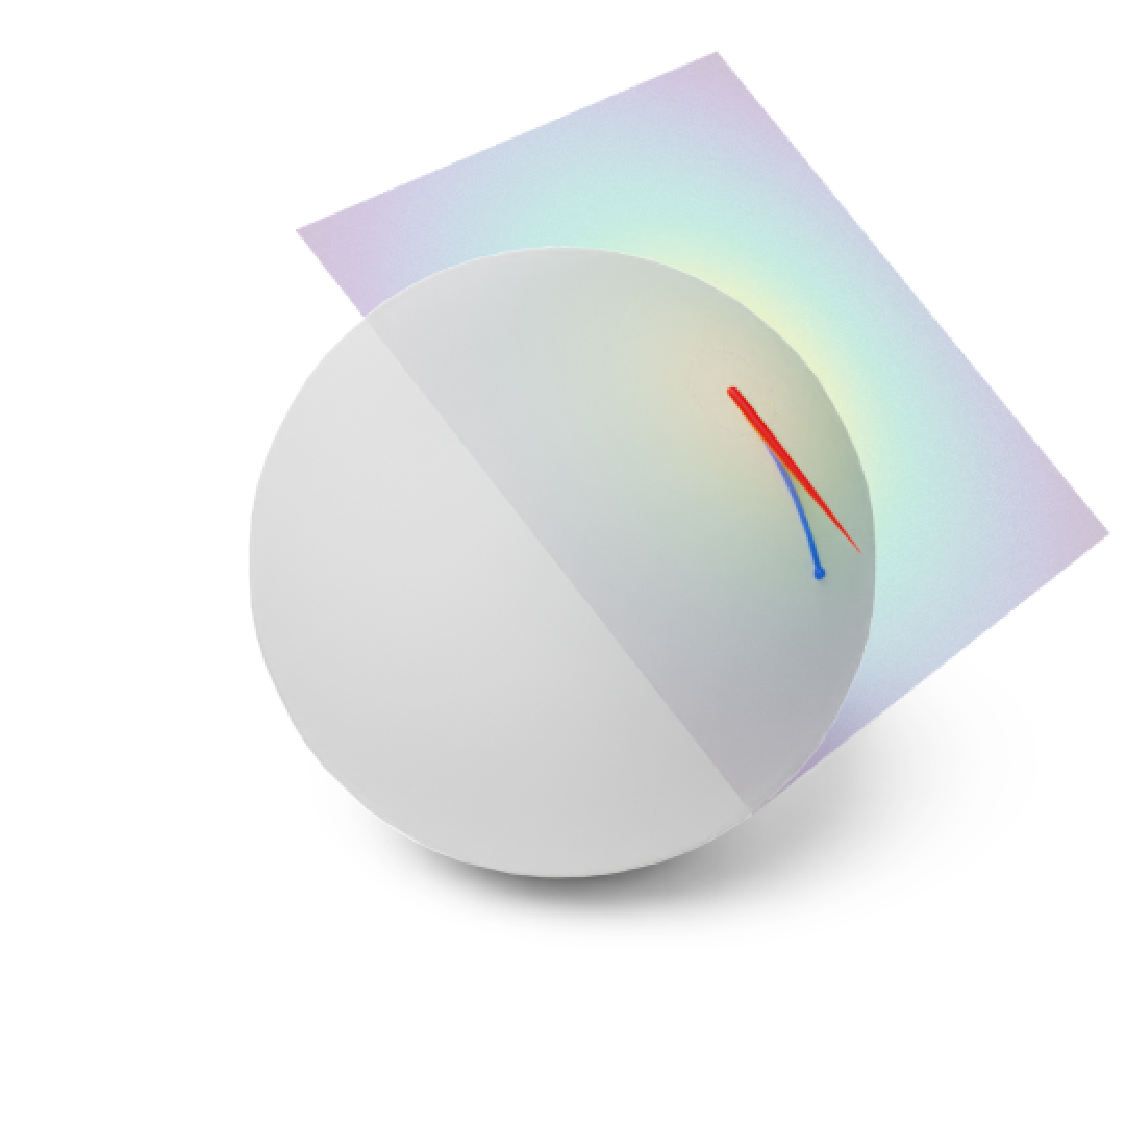
\includegraphics[width=\textwidth, trim={4.5em 4.5em 0em 0em},clip]{images/rsgm/grw_step.pdf}
		\caption{A single step of a Geodesic Random Walk.}
	\end{subfigure}
	\hfill
	\begin{subfigure}[t]{0.24\textwidth}
		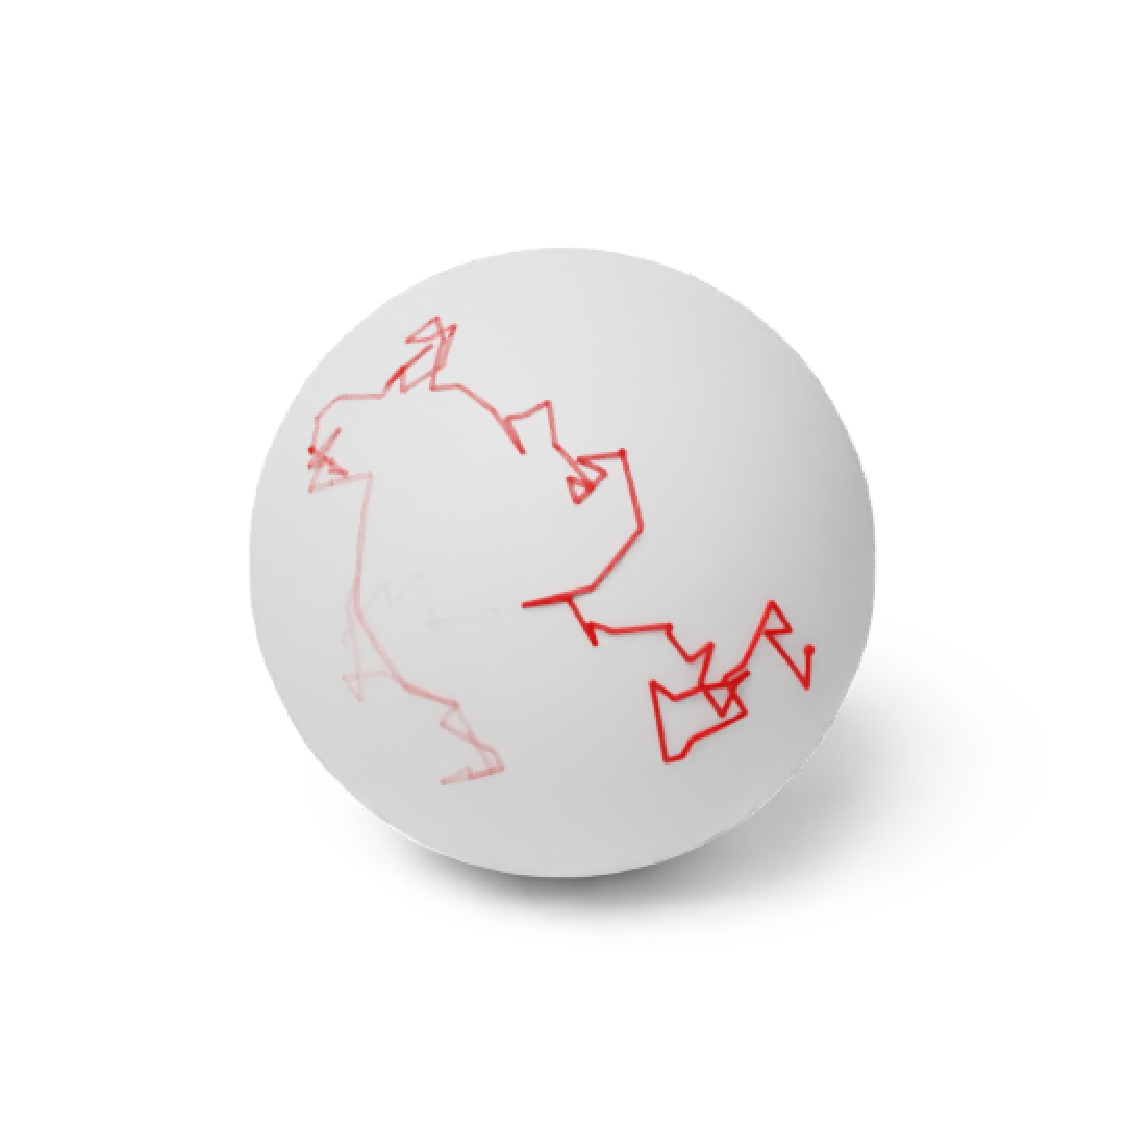
\includegraphics[width=\textwidth, trim={2.5em 4.5em 2.0em 0em},clip]{images/rsgm/grw.pdf}
		\caption{Many steps yield an approximate trajectory.}
	\end{subfigure}
	\hfill
	\begin{subfigure}[t]{0.48\textwidth}
		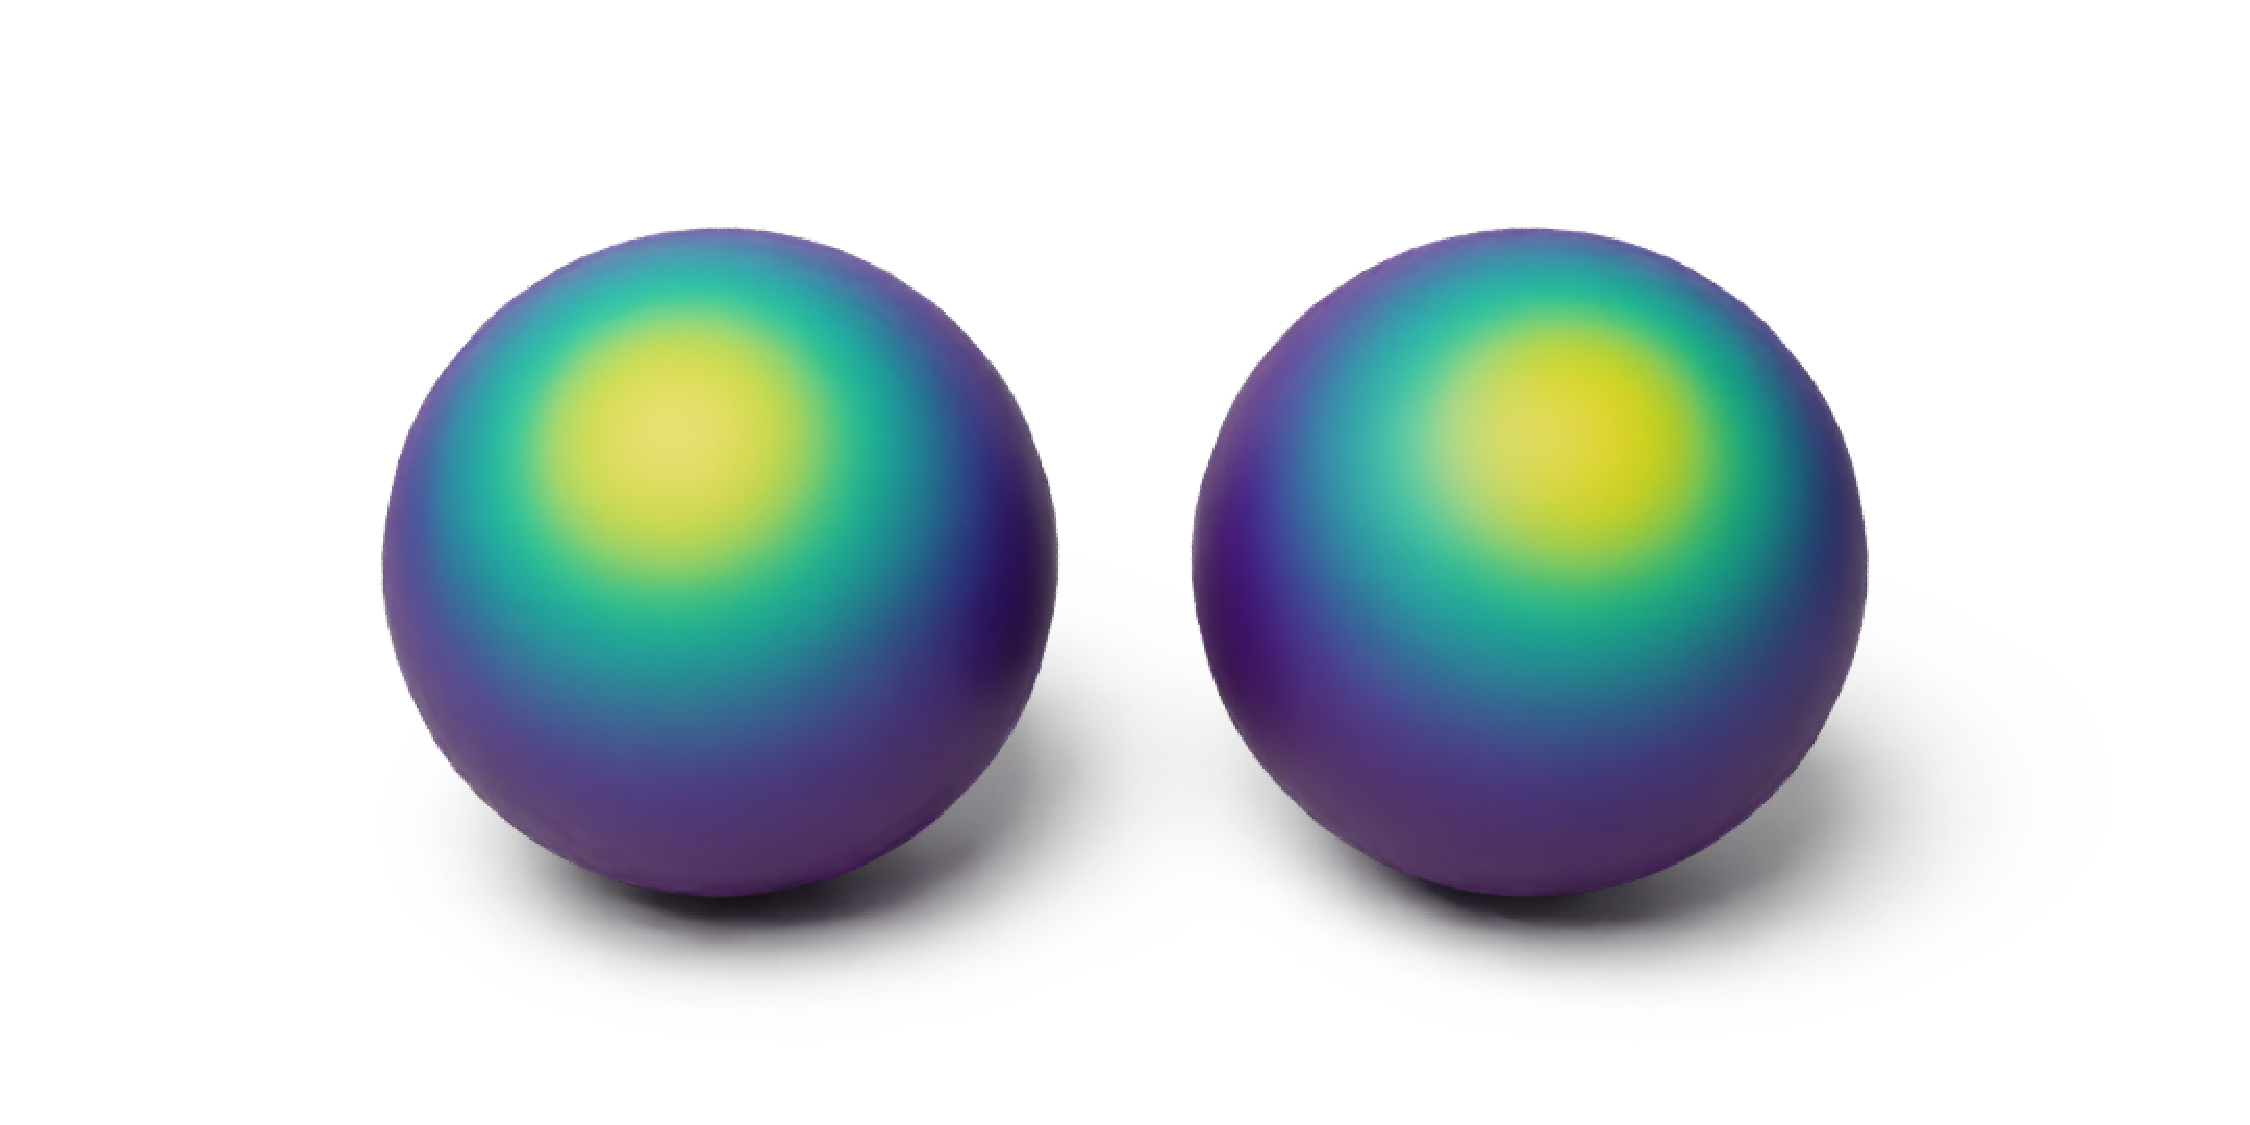
\includegraphics[width=\textwidth, trim={2.5em 2.5em 2.5em 2.5em},clip]{images/rsgm/sigma_0.51.pdf}
		\caption{Gaussian random walk [Left] and the Brownian motion density [Right] agree well for small time steps.}
	\end{subfigure}
	\caption{Geodesic random walks can be used to approximate Brownian motion and more generally SDEs on manifolds. (a) At each step, tangential noise is sampled (red), which is added the drift term (not pictured).
		This tangent vector is then pushed through the exponential map to produce a geodesics step on the manifold (blue).
		(b) Iterating this procedure yield approximate sample paths from the process.
	}
	\label{fig:grw}
\end{figure*}

Obtaining samples from SDEs on a manifold is non-trivial in general.
As in the Euclidean case, we cannot sample the continuous time dynamics of a manifold valued stochasitc process, and so must resort to finite time setp approximations.

The simplest approach would be to apply the Euclidean space techiniques of \cref{sec:approximate_sde_sampling} to sample Euclidean stochasitc diferential eqautions by embedding the manifold into Euclidean space, an \emph{extrinsic} approach.
We know that the manifold valued stochasitc differential equations can be realised as a Euclidean stochasitc differential equations (\cref{sec:embedded_manifold_sdes}) that stick to the surface of the manifold through time.
Unfortunatly with a discrete step size, the discretisation is guarenteed almost surely to leave the surface of the manifold, where the process becomes defined.
While this can be corrected by taking small step sizes and projecting samples back onto the surface of the manifold, these projections can be expensive and the procedure inaccurate.
It also requries choosing an embedding for the manifold at hand and finding the form of the projection function.

Here instead we consider an \emph{intrisic} approach based on geodesic random walks, see \textcite{jorgensen1975central} for a review of their properties.
Geodesic random walks can approximate \emph{any} well-behaved diffusion on \(\c{M}\).
Hence, we introduce them in a general framework and consider discretisations of a \(\c{M}\)-valued stochasitc differential equation.
This generalisation is key to sampling the backward diffusion process defined in \Cref{thm:time_reversal_manifold}.

\begin{definition}[Geodesic random walk]
	Let \(\v{X}^\gamma_0 \sim p_0\) be a \(\c{M}\)-valued random variable.
	Let \(\v{b}: \R^+ \x \c{M} \to T\c{M}\) be a drift function and \(\sigma: \R^+ \to \R^+\) a noise term.

	For any \(\gamma > 0\), we define \((\v{X}_n^\gamma)_{n \in \N, n > 0}\) such that
	\[
		\v{X}_{n+1}^\gamma = \exp_{X_{n}^\gamma}\sbr{\gamma \sbr{ b(X_{n}^\gamma) + \sqrt{\gamma} V_{n+1} }}
	\], 
	where \((V_n)_{n \in \N}\) is a sequence of \(T_{\v{X}_n^\gamma}\c{M}\)-valued random variables such that for any \(n \in \N\), 
	\[
		\E\sbrvert{V_{n+1}}{\c{F}_n} = 0 \text{ and }\E\sbrvert{V_{n+1} V_{n+1}^\top}{\c{F}_n} = \sigma \sigma^\top
	\], 
	where \(\c{F}_n\) is the filtration generated by \(\cbr{\v{X}_k^\gamma}_{k=0}^n\).

	We say that the \(\c{M}\)-valued process \((\v{X}_n^\gamma)_{n \in \N}\) is a geodesic random walk.
\end{definition}
This definition gives us a clear blueprint to sample \(\c{M}\)-vauled stochasitc differential equations.
Let 
\[
	\d\v{X}_t = \v{b}(t, \v{X}_t) \d t + \sigma(t) \d\v{B}_t, \quad \v{X}_0 \sim p_0	
\]
be an \(\c{M}\)-valued stochasitc differetial equation.
We initialise the geodesic random walk with \(\v{X}_0^\gamma\sim p_0\), and then iterate the geodesic random walk using the drift and noise coefficients of the stochasitc differential equation.

\Cref{alg:grw_rsgm} summarises the implementation of this algorithm for sampling the stochasitc differenital equation.
\Cref{fig:grw} provides a graphical illustration of this procedure.

Importantly, there are results avaliable for this scheme that guarentee a certain level of accuracy. 
For eaxmple, see \textcite{kuwada2012convergence,cheng2022theorymanifold} for quantitative error bounds in the time-homogeneous
case.
These error bound depend on a number of constants enocoding the curvature of the manifold, but importantly in order to ensure that the expected distance between the approximate dynamics and the continuous time dynamics are bounded by \(\epsilon\), one needs to use a number of discretisation setep sthat scales with \(\frac{1}{\epsilon^2}\).
This rate is the same order as required to achive the same accuracy with Euler-Murayama discresitation of Eucldiean stochasitc differential equations, and so we do not lose any samplign efficiency by being in the manifold setting.
We can therefore, with increasing numbers of steps, obtain arbitrary precision for the use case we have.

In addtion, we extend these results to cover the time-inhomogeneous setting that we use in diffusion modelled. See \cref{sec:discr-bounds-grw} for these results.

\begin{algorithm}[!t]
	\caption{\small GRW (Geodesic Random Walk)}
	\label{alg:grw_rsgm}
	\begin{algorithmic}[1]
		\small
		\Require \(T, N, X_0^\gamma, b, \sigma, \mathrm{P}\)
		\State \(\gamma = T / N\) \Comment Step-size
		\For{\(k \in \{0, \dots, N-1\}\)}
		\State \(Z_{k+1} \sim \mathrm{N}(0, \m{I})\) \Comment Sample a Gaussian in the tangent space of \(X_{k}^\gamma\)
		\State \(W_{k+1} = \gamma b(k \gamma, X_k^\gamma) + \sqrt{\gamma} \sigma(k \gamma, X_k^\gamma) Z_{k+1}\) \Comment Compute the Euler--Maruyama step on tangent space
		\State \(X_{k+1}^\gamma = \exp_{X_k^\gamma}[W_{k+1}]\) \Comment Move along the geodesic defined by \(W_{k+1}\) and \(X_{k}^\gamma\) on \(\c{M}\)
		\EndFor
		\State {\bfseries return} \(\{ X_k^\gamma\}_{k=0}^{N}\)
	\end{algorithmic}
\end{algorithm}

\subsection{Predictor-corrector scheme}
\label{sec:predictor-corrector}
\todo{fix up}
In addition to presenting geodesic random walks as a general framework for discretising stochasitc diferential equations on manifolds, in this section we present a predictor-corrector scheme, adapting the techniques of \textcite{allgower2012numerical,song2020score} to the manifold setting.

Changes between \Cref{alg:grw_rsgm} and \Cref{alg:grw-c} are highlighted in red.
Let \(t \in \sbr{0,T}\), \(\gamma >0\) and \(k = \floor{t / \gamma}\).
We remark that \Cref{alg:grw-c} corresponds to the recursion associated with \((X_j^{t,\gamma})_{j \in \N}\) such that for any \(j \in \N\) \begin{equation} X_{j+1}^{t,\gamma} = \exp_{X_j^{t,\gamma}}[\tfrac{\gamma}{2} \nabla \log p_{T-k\gamma}(X_j^{t,\gamma}) + \sqrt{\gamma} Z_{j+1}] , \end{equation} where \(\{\bar{Z}_j\}_{j \in \N}\) is a family of i.i.d Gaussian random variables with zero mean and identity covariances matrix in \(\R^p\) and for any \(j \in \N\), \(Z_j = \mathrm{P}(X_j^{t,\gamma}) \bar{Z}_j\).
Note that here \(k \in \{0, N-1\}\) is fixed.
Letting \(\gamma \to 0\), we obtain that under mild assumptions, see \cite[Theorem 3.1]{kuwada2012convergence}, \((X_j^{t, \gamma})_{j \in \N}\) converges to \((\v{X}_s^t)_{s \geq 0}\) such that \begin{equation} \mathrm{d} \v{X}_s^t = \tfrac{1}{2} \nabla \log p_{T-t}(\v{X}_s^t) \mathrm{d} s + \mathrm{d} \v{b}_s^\c{M} .
\end{equation}
We have that \(p_{T-t}\) is the invariant measure of \((\v{X}_s^t)_{s \geq 0}\).
Hence, the role of the corrector step is to project the distribution back onto \(p_{T-t}\) for all times \(t \in \sbr{0,T}\), see \Cref{fig:illustration_pred_correc}.
\begin{figure}[htb]
	\centering
	\begin{tikzpicture}
		\draw [stealth-, line width = .05cm] (0,0) .. controls  (2,-4) and (4,4) .. (6,0);
		\draw [-stealth, line width = .05cm, blue!50!black, dashed] (0,0) -- (1.3,-2.3);
		\draw [-stealth, line width = .05cm, red!50!black, dashed] (1.3,-2.3) -- (1.3,-1.2);
		\draw [-stealth, line width = .05cm, blue!50!black, dashed] (1.3,-1.2) -- (2.8,-0.7);
		\draw [-stealth, line width = .05cm, red!50!black, dashed] (2.8,-0.7) -- (2.6, -0.5);
		\node [below=0.2cm] at (6,0) {\(p_{\textrm{data}}\)};
		\node [left=0.3cm] at (0,0) {\(\mathcal{L}(X_0^\gamma) = p_T\)};
		\node [below=0.2cm] at (1.3,-2.3) {\(\mathcal{L}(X_{1/2}^\gamma)\)};
		\node [below right=0.1cm] at (1.3,-1.2) {\(\mathcal{L}(X_{1}^\gamma)\)};
		\node [right=0.2cm] at (2.8,-0.7) {\(\mathcal{L}(X_{3/2}^\gamma)\)};
		\node [above left=0.1cm] at (2.6, -0.5) {\(\mathcal{L}(X_{2}^\gamma)\)};
	\end{tikzpicture}
	\caption{Illustration of the effect of the corrector step on RSGM.
		The black line corresponds to the dynamics of the noising process \((p_t)_{t \in \sbr{0,T}}\).
		The blue dashed lines correspond to the predictor step (going backward in time) and the red dashed lines correspond to the corrector step (projecting back onto the initial dynamics).
		Note that \(\mathcal{L}(X_1^\gamma) \approx p_{T- \gamma}\) and \(\mathcal{L}(X_2^\gamma) \approx p_{T- 2\gamma}\).
	}
	\label{fig:illustration_pred_correc}
\end{figure}

\begin{algorithm}[!ht]
	\caption{\small GRW-c (Geodesic Random Walk with corrector)}
	\label{alg:grw-c}
	\begin{algorithmic}[1]
		\small
		\Require \(T, N, X_0^\gamma, b, \sigma, \mathrm{P}\)
		\State \(\gamma = T / N\) \Comment Step-size
		\For{\(k \in \{0, \dots, N-1\}\)}
		\State \textcolor{blue!50!black}{/// PREDICTOR STEP}
		\State \textcolor{blue!50!black}{\(\bar{Z}_{k+1/2} \sim \mathrm{N}(0, \mathrm{I}_p)\)} \Comment Standard Gaussian in ambient space \(\R^p\)
		\State \textcolor{blue!50!black}{\(Z_{k+1/2} = \mathrm{P}(X_k^\gamma) \bar{Z}_{k+1/2}\)} \Comment Projection in the tangent space \(\mathrm{T}_x \c{M}\)
		\State \textcolor{blue!50!black}{\(W_{k+1/2} = \gamma b(k \gamma, X_k^\gamma) + \sqrt{\gamma} \sigma(k \gamma, X_k^\gamma) Z_{k+1/2}\)} \Comment Euler--Maruyama step on tangent space
		\State \textcolor{blue!50!black}{\(X_{k+1/2}^\gamma = \exp_{X_k^\gamma}[W_{k+1/2}]\)} \Comment Geodesic projection onto \(\c{M}\)
		\State \textcolor{red!50!black}{/// CORRECTOR STEP}
		\State \textcolor{red!50!black}{\(\bar{Z}_{k+1} \sim \mathrm{N}(0, \mathrm{I}_p)\)} \Comment Standard Gaussian in ambient space \(\R^p\)
		\State \textcolor{red!50!black}{\(Z_{k+1} = \mathrm{P}(X_{k+1/2}^\gamma) \bar{Z}_{k+1}\)} \Comment Projection in the tangent space \(\mathrm{T}_x \c{M}\)
		\State \textcolor{red!50!black}{\(W_{k+1} = \tfrac{\gamma}{2} b(k \gamma, X_{k+1/2}^\gamma) + \sqrt{\gamma} \sigma(k \gamma, X_{k+1/2}^\gamma) Z_{k+1}\)} \Comment Euler--Maruyama step on tangent space \label{line:dete}
		\State \textcolor{red!50!black}{\(X_{k+1}^\gamma = \exp_{X_{k+1/2}^\gamma}[W_{k+1}]\)} \Comment Geodesic projection onto \(\c{M}\)
		\EndFor
		\State {\bfseries return} \(\{ X_k^\gamma\}_{k=0}^{N}\)
	\end{algorithmic}
\end{algorithm}

% \begin{algorithm}[!t]
% 	\caption{\small RSGM-c (Riemannian Score-Based Generative Model with corrector)}
% 	\label{alg:rsgm-c}
% 	\begin{algorithmic}[1]
% 		\small
% 		\Require \(\varepsilon, T, N, \{X_0^m\}_{m=1}^M, \mathrm{loss}, \mathbf{s}, \theta_0, N_{\textrm{iter}}, p_{\t{ref}}, \mathrm{P}\)
% 		\State{{/// TRAINING ///}}

% 		\For{\(n \in \{0, \dots, N_{\textrm{iter}}-1\}\)}
% 		\State \(X_0 \sim (1/M) \sum_{m=1}^M \delta_{X_0^m}\) \Comment Random mini-batch from dataset
% 		\State \(t \sim U(\sbr{\varepsilon, T})\) \Comment Uniform sampling between \(\varepsilon\) and \(T\)
% 		\State \(\v{X}_t = \textrm{GRW}(t, N, X_0, 0, \m{I}, \mathrm{P})\) \Comment Approximate forward diffusion with \cref{alg:grw_rsgm}

% 		\State
% 		\(\ell(\theta_n) = \ell_t(T, N, X_0, \v{X}_t, \mathrm{loss}, \mathbf{s}_{\theta_n})\)
% 		\Comment Compute score matching loss from \cref{tab:sm_losses} \State
% 		\(\theta_{n+1} = \verb|optimizer_update|(\theta_n, \ell(\theta_n))\) \Comment ADAM
% 		optimizer step
% 		\EndFor \State \(\theta^\star = \theta_{N_{\textrm{epoch}}}\)
% 		\State{{/// SAMPLING ///}} \State \(Y_0 \sim p_{\t{ref}}\) \Comment
% 		Sample from uniform distribution \State
% 		\(b_\theta^\star(t, x) = \mathbf{s}_{\theta^\star}(T-t, x)\) for any
% 		\(t \in \sbr{0,T}\), \(x \in \c{M}\) \Comment Reverse process drift \State
% 		$\{Y_k\}_{k=0}^{N} = \textrm{GRW-c}(T, N, Y_0, b_{\theta^\star}, \m{I},
% 			\mathrm{P})$ \Comment Approximate reverse diffusion with \Cref{alg:grw-c} \State
% 		{\bfseries return} \(\theta^\star, \{Y_k\}_{k=0}^{N}\)
% 	\end{algorithmic}
% \end{algorithm}

\subsection{Score approximation on Riemannian manifolds}
\label{sec:riem-score-appr}

As with the time reveral in the Euclidean setting, the reverse process from \cref{eq:time_reversal_manifold} involves the Stein score \(\nabla \log p_t\) of the stochasitc differetial equation.
We will need to again approximate this quantity through a score matching loss.

In this section we will assume that we have a \(\c{M}\)-valued stochasitc process \(\del{\v{X}_t}_{t\in\sbr{0, T}}\) defined by
\[
	\d\v{X}_t = \v{b}(t, \v{X}_t) \d t + \sigma(t) \d\v{B}_t, \quad \v{X}_0 \sim p_0	
\].
We will denote \(p_t\) as the marginal denisty of \(\v{X}_t\) and \(p_{s,t}\) the joint denisty of \(\v{X}_s\) and \(\v{X}_t\) for some \(t>s \geq 0\), relative to the Riemannian volume form and the product Riemanian volume forms respectivly, and \(\P_t\) and \(\P_{t|s}\) be their distributions.
We will let \(\v{s}: \R^+ \x \c{M}\to T\c{M}\) be an arbirtray smooth time-varying vector field on \(\c{M}\), representing the approximation we learn to the score function.

The \emphhyperref{denoising score matching}{def:dsm} loss carries over naturally to the manifold setting, nothing about its derivation rpesetns difficulties when transiting to more general geometries.
In the manifold setting the denoising score matching loss \(\ell_{t|s}\) is given by
\[
	\ell_{t|s}(\v{s}) = \int_{\c{M}^2} \norm{\v{s}(t, \v{X}_t) - \nabla_{\v{X}_t} \log p_{t|s}\delvert{\v{X}_t}{\v{X}_s}}_g^2 \; p_{s,t}(\v{X}_t, \v{X}_s)\d\v{X}_s\d\v{X}_t
\]
where \(\norm{\cdot}_g\) is the \emphhyperref{Riemannain norm}{def:riemannian_norm} and \(\d\v{X}_s\) is shorthand for integrating against the \emphhyperref{Riemannian volume measure}{def:riemannain_volume_measure}, \(\d\vol_g(\v{X}_s)\).
Unfortunatly however, on general gemoetries, for the foreward noising processes given by taking Langenvin dynamics with either the Riemannian normal distribtion or the wrapped Gaussian distribution the forward transition kernels, \(p_{t|0}\), do not have accessable analytic forms.
This makes application of the denoising score matching loss on general geometries difficult unless the specific manifold and foreward noising process in question has a tractable form.

We instead turn to \emphhyperref{implicit score matching}{def:ism} as this avoids needing access to the forward transition kernel.
The derivation of the implicit score matching loss does not carry over to the manifold setting as it uses calculs results specific to the Euclidean setting.
Here we prove a version of the implicit score matching result suitable for manifolds.
\begin{proposition}[Manifold implicit score matching]
	\label{prop:manifold_ism}
	Let \(t, s \in \ocbr{0, T}\) with \(t > s\).
	Under sufficient regualrity conditions of the product \(p_{t|s}(\v{X}_t | \v{X}_s) \v{s}(t, \v{X}_t)\),
	\[
		\ell_{t|s}(\v{s}_t) = 2 \ell^{ism}(\v{s}_t) + \int_{\c{M}^2} \norm{\nabla_{\v{X}_t}\log p_{t|s}(\v{X}_t | \v{X}_s) }_g^2 \; p_{s,t}(\v{X}_s, \v{X}_t) \d\v{X}_s\d\v{X}_t
	\]
	where \(\ell^{ism}(\v{s}_t)\) is given by
	\[
		\ell^{ism}(\v{s}_t) = \int_{\c{M}} \sbr{\frac{1}{2}\norm{\v{s}_t(\v{V}_t)}_g^2 + \dive_g(\v{s}_t)(\v{X}_t)} p_t(\v{X}_t) \d\v{X}_t	
	\]
	where \(\norm{\cdot}_g\) is the Riemannain norm and \(\dive_g\) the Riemannian divergence.
\end{proposition}
The proof of this proposition is delayed to \cref{sec:manifold_ism_proof}.
The main difference from the Euclidean case is the application of manifold divergence theorems on non-compact manifolds \parencite{gaffney1954}.
The regularity conditions on \(p_{t|s}(\v{X}_t | \v{X}_s) \v{s}(t, \v{X}_t)\) require that this product, its absolute value, and its determinant are \(L_1\) integrable, a very mild condition usually satisfied by the field decaying suitably fast away from some point.

Since the second term is independent of \(\v{s}_t\)r  for any \(t \in \ocbr{0,T}\), the minimizers of the loss \(\ell^{ism}_t\) on \(\Gamma(T\c{X})\)  are the same as the ones for \(\ell_{t|s}\).

The Riemannain divergence of an arbirtray vector field can be achived in an automatic differentiation package by using the coordinate expression for the divergence in a chart \((\phi, U)\), see \cref{def:riemannain_divergence_chart},
\[\dive V = \frac{1}{\sqrt{\det g}} \partial\phi_i \del{\sqrt{\det g}\; V_i}\label{eq:riemannian_divergence_coords}\].
The \(\partial\phi_i \del{\sqrt{\det g}\; V_i}\) part can be intepreted as the Euclidean divergence of the vector field \[V(\phi_1, ..., \phi_n) = \begin{bmatrix}
	\sqrt{\det g(\phi_1, ..., \phi_n)}\; V_1 (\phi_1, ..., \phi_n) \\ \vdots \\ \sqrt{\det g(\phi_1, ..., \phi_n)}\; V_n (\phi_1, ..., \phi_n)
\end{bmatrix}\label{eq:euclidean_riamannian_divergence}\],
and this can be computed by an automatic differetiaiton package if we have the expression for the metric and the components of the vector field in the chart.

As in the Euclidean case the computation of a divergence in an automatic differentation package requres \(d\) Jacobian-vector calls.
This can again be sped up with Hutchinson's trace trick \parencite{hutchinson1989stochastic} by applying it to the computation of the Euclidean divergence component of \cref{eq:euclidean_riamannian_divergence}. 

Again as in the Eucldiean case and following \textcite{song2020improved, nichol2021improved}, these losses work only for a single time \(t\). The losses are therefore integrated over time and can be weighted with a term \(\lambda_t > 0\).

\subsection{Parametric family of vector fields.}
Finally, we need to choose a method to approximate \((\nabla \log p_t)_{t \in \sbr{0,T}}\) by a parametrised function \(\mathbf{s}_\theta\), \(\mathbf{s}_\theta: \sbr{0,T} \to \Gamma(T\c{M})\), that is differentiable with respect to its parameters.
In addition, under the assumption that \(p_t\) is a smooth density, we know that the score function \(\nabla \log p_t\) will itself be a smooth vector field.
With this in mind we want to parametrise the score function in a smooth, or at least continuous, manner to prevent any large discontinuities in the learnt score function.

The general stratergy shall be to parametrise a vector field as a finite sum of some basis fields, weighted by smooth functions on the manifold.
That is,
\[
	V = f^i E_i, \quad f_i \in C^\infty(\c{M}), \; E_i \in \Gamma(T\c{M})	
\].
In \(d\)-dimension Euclidean space there exists a set of \(d\) smooth basis fields \((E_i)_{i=1}^d\) which space the tangent sapce, as it is \emphhyperref{parallisable}{}, creating a bijection between the tanget bundle and \(C^\infty(\c{M}, \R^d)\).
We can then express the score function as \[\v{s}_\theta(\v{X})\sum_{i=1}^d \bar{\v{s}}^i_\theta(\v{X}) E_i(\v{X})\label{eq:score_function_basis_expression}\] where \(\bar{\v{s}}_\theta \in C^\infty(\c{M}, \R^d)\).
This is not true in general for manifolds, most are \emphhyperref{non-parallisable}{}, and the space of vector fields forms a module, not a vector space (see \cref{def:}).

Fortunately however the space of vector fields is \emphhyperref{finitely generated}{} for any Riemannian manifold.
One can rely therefore on a larger set of smooth vector fields \(\{E_i(x)\}_{i=1}^n\) with \(n > d\) that \emph{does} span the tangent bundle.
This does not create a bijection between the tangent bundle and \(C^\infty(\c{M}, \R^n)\), but does create an injection, so any vector field can be represented.
Then it suffices to construct a smooth neural network \(\bar{\v{s}}_\theta: \sbr{0, T} \times \c{M} \rightarrow \R^n\) to parametrise the score network as \[\v{s}_\theta(t,x) = \sum_{i=1}^n \bar{\v{s}}^i_\theta(t,\v{X}) E_i(x)\].
There are a number of ways we can choose the generating sets \(\{E_i(\v{X})\}_{i=1}^n\).

Most simply, we can use \emphmarginnote{projected vector fields}.
Let \(\c{M}\) be a smooth embedded submanifold of \(\R^n\), and let \(\inclusion: \c{M}\to \R^n\) be the inclusion map that preserves the Riemannain metric between \(\c{M}\) and \(\R^n\).
This is guarenteed to exist by the \emphhyperref{Nash embedding theorem}{thm:nash-embed-thm}.
For every vector field \(V\in \Gamma(T\c{M})\), there is a vector field in \(V'\in\Gamma(T\R^n)\) that when \emphhyperref{restricted}{} to \(\inclusion(\c{M})\) is \emphhyperref{\(\inclusion\)-related}{} to \(V\).
The converse is not true however.
It is only true if the vector field \(V'\) is \emphhyperref{tangent}{} to \(\inclusion(\c{M})\), \textcite[see]{lee2013smooth}.

The Riemannain gradients of the inclusion map, \(\grad_g \inclusion_i\), generate the tangent bundle of \(\c{M}\) and can therefore be used to parametrise vector fields. \textcite{forr}


More concretly, if we define \(\bar{\v{s}}_\theta: [0,T] \x \c{M} \to T\R^n\) then we can define the parametrised score function as
\[\v{s}_\theta(t, \v{X}) = (\d F)^{-1} \sbr{\proj_{\d F(T\c{M})} \bar{\v{s}}_\theta(t, \v{X})}\].
This is equivalent to taking the Euclidean basis fields, \((E_i)_{i=1}^n\) and defining the score function as
\[\v{s}_\theta(t,x) = \sum_{i=1}^n \bar{\v{s}}^i_\theta(t,\v{X})\proj_{\d F(T\c{M})} (\d F)^{-1}\sbr{ E_i(\v{X}) }\]. One attractive property of this construction is that for a vector field \(V\in \Gamma{T\c{M}}\), 
\[\dive_g V = \dive \d F (V)\], where on the right hand side this is the usual Euclidean divergence, and so we can avoid the complexity of \cref{eq:riemannian_divergence_coords} and compute the divergence of the vector field in Eucldiean space with regular automatic differentiation.

For any Lie group \(G\) we can use a set of \emphmarginnote{divergence-free vector fields}.
We can immediatly use a global basis of smooth frames of size \(d\) as Lie groups are parallizable.
This is immediatly useful as we can define a smooth score function using \(d\) basis fields.
More usefuly, we can construct this basis to be \emph{divergence free}.

To construct this let \[L_g: G\to G, \quad L_g(g') = g\cdot g'\] the left translation of a Lie group.
We call a vector field \(V\in \Gamma(TG\) on a Lie group left-invariant if
\[(\d L_g)_{g'} (V_{g'} = V_{g\cdot g'})\].
For any vector \(v\in T_eG\), where \(e\in G\) is the identity element, there exists a left-invariant vector field \(V\in \Gamma(TG)\) \parencite[Chapter 8]{lee2013smooth}.
We can thererfore use any basis of \(T_e G\), \((v_i)_{i=1}^n\), to create a left-invariant global basis of \(\Gamma(TG)\), \((E_i)_{i=1}^d\) such that \(E_i(e) - v_i\).

As a result of the left invariance of the basis fields, we have that for any \(i \in \{1, \dots, d\}\), \(\dive_g(E_i)=0\).
This result simplifies the computation of \(\dive_g(\v{s}_\theta)\) where \(\v{s}_\theta\) is of the form of \cref{eq:score_function_basis_expression} since we have that \[\dive_g (\v{s}_\theta)(t, \v{X}) &= \sum_{i=1}^d E_i(\v{s}^i_\theta)(t, \v{X}) + \sum_{i=1}^d \v{s}^i_\theta(t,\v{X}) \dive_g (E_i)(\v{X}) \\&= \sum_{i=1}^d \d \v{s}^i_\theta (E_i)(t, \v{X}) \], and \(\d \v{s}^i_\theta\) can be computed with automatic differentiation and \emphhyperref{lowering an index}{{def:lowering_an_index}}, \cite[see][]{falorsi2020neural}.
Note that this simplified divergence computation can be extended to any homogeneous space of \(G\) by projecting the divergence free vector fields from the Lie group onto the homogenous space, where they remain divergence free.

Finally, and least elegantly, we can use \emphmarginnote{coordinates vector fields}.
If we can choose a chart \((\phi, U)\) such that it covers the manifold expcept for a set of measure zero, we can parametrise the score function in these local coordinates.
We can define a set of local vector fields \(\{E_i\}_{i=1}^d = \{\partial_i \phi\}_{i=1}^d\) .
These will not span the full tangent bundle, but they will span the tangent space expcept on a set of points we will, by virture of the set being measure zero, never encounter in practise.
Note however, these fields may nto be smooth or continuous at certain points, and so present issue with the smoothenss or continuity of the score function.
The sphere presents two possible examples of this approach.
Firstly we could use a latitude-longitde chart.
This coordinate system is not defined at the poles, or along a line joining them.
However, the vector fields produced are for all practcal purposes smooth across this seam, and wo work well.
An alternaive would be to use polar coordinates.
These are only undefine at a single pole and so also present a viable option.

Combining this parameterization with the score matching losses, the time-reversal formula of \cref{thm:time_reversal_manifold} and the sampling of forward and backward processes described in \cref{sec:geodesic_random_walk}, we define our RGSM algorithm in \cref{alg:rsgm}.
This algorithm can also benefit from a predictor-corrector scheme as in \textcite{song2020score}, see \Cref{sec:predictor-corrector}.

\begin{algorithm}[!t]
	\caption{\small RSGM (Riemannian Score-Based Generative Model)}
	\label{alg:rsgm}
	\begin{algorithmic}[1]
		\small
		\Require \(\varepsilon, T, N, \{X_0^m\}_{m=1}^M, \mathrm{loss}, \mathbf{s}, \theta_0, N_{\textrm{iter}}, p_{\textup{inv}}, \mathrm{P}\)
		\State{/// TRAINING ///}

		\For{\(n \in \{0, \dots, N_{\textrm{iter}}-1\}\)}
		\State \(X_0 \sim (1/M) \sum_{m=1}^M \delta_{X_0^m}\) \Comment Random mini-batch from dataset
		\State \(t \sim U(\sbr{\varepsilon, T})\) \Comment Uniform sampling between \(\varepsilon\) and \(T\)
		\State \(\v{X}_t = \textrm{GRW}(t, N, X_0, b, \m{I}, \mathrm{P})\) \Comment Approximate forward diffusion with \cref{alg:grw_rsgm}
		\State \(\ell(\theta_n) = \ell_t(T, N, X_0, \v{X}_t, \mathrm{loss}, \mathbf{s}_{\theta_n})\) \Comment Compute score matching loss from \cref{tab:sm_losses}
		\State \(\theta_{n+1} = \verb|optimizer_update|(\theta_n, \ell(\theta_n))\) \Comment ADAM optimizer step
		\EndFor
		\State \(\theta^\star = \theta_{N_{\textrm{epoch}}}\)
		\State{/// SAMPLING ///}
		\State \(Y_0 \sim p_{\textup{inv}}\) \Comment Sample from uniform distribution
		\State \(b_\theta^\star(t, x) = \mathbf{s}_{\theta^\star}(T-t, x)\) for any \(t \in \sbr{0,T}\), \(x \in \c{M}\) \Comment Reverse process drift
		\State \(\{Y_k\}_{k=0}^{N} = \textrm{GRW}(T, N, Y_0, b_{\theta^\star}, \m{I}, \mathrm{P})\) \Comment Approximate reverse diffusion with \Cref{alg:grw_rsgm}
		\State {\bfseries return} \(\theta^\star, \{Y_k\}_{k=0}^{N}\)
	\end{algorithmic}
\end{algorithm}

\section{Riemannian Score-Based Generative Modelling on Compact Manifolds}

\label{sec:compact}

Assuming compactness of the manifold \(\c{M}\), we can leverage a number of special properties to implement a specific case of our algorithm.

\subsection{Forward noising process}

In the compact case, for the distribtion we target in the forward noising process, we can choose \(U(x) = 0\), giving simple Brownian motion, \[ \d \v{X}_t = \d\v{B}_t^M\].
This will converge to a density proportional to the Riemannian volume form, simply the \emphmarginnote{uniform distribution on a compact manifold} given by \(\mu = \frac{\vol_g}{\int_\c{M} \vol_g} \).
This is well-defined as a compact manifold has finite volume.
Regardless of the starting distribution the SDE will converge to the uniform distribution exponentially quickly.\todo{cite}

\subsection{Learning the score}

Targeting the uniform distribution is additionally useful as the transition kernel of the resulting Langevin stochasitc differential eqaution is the heat kernel.

Contrary to the Gaussian transition density of Brownian motion in the Euclidean setting, it is typically only available as an infinite series on compact manifolds.

In order to circumvent this issue we consider two techniques: \begin{enumerate*}[label=\roman*)] \item a truncation of the Sturm--Liouville decomposition, \item a Taylor expansion around \(t=0\) called a Varadhan asymptotics.
\end{enumerate*}

\subsubsection{Sturm--Liouville decomposition}
In the case of compact manifolds the heat kernel can be represented by a \emphmarginnote{Sturm--Liouville decomposition} \parencite{chavel1984eigenvalues}, given for any \(t > 0\) and \(x_0, x_t \in \c{M}\) by \[ \label{eq:infinite_sum1} {p_{t|0}(x_t|x_0) = \sum_{j \in \N} \mathrm{e}^{-\lambda_j t} \phi_j(x_0)\phi_j(x_t),} \] where the convergence occurs in \(\mathrm{L}^2(p_{\textup{inv}} \otimes p_{\textup{inv}})\), and \((\lambda_j)_{j \in \N}\) and \((\phi_j)_{j \in \N}\) are the eigenvalues, respectively the eigenvectors of \(-\Delta_g\), the Laplace-Beltrami operator on the manifold \cite[Section 2]{saloff1994precise}.
When the eigenvalues and eigenvectors are known, we rely on an approximation of the logarithmic gradient of \(p_{t|0}\) by truncating the sum in \cref{eq:infinite_sum1} with \(J \in \N\) terms to obtain for any \(t > 0\) and \(x_0,x_t \in \c{M}\) \begin{equation} \label{eq:heat_kernel_trunc} \nabla_{x_t} \log p_{t|0}(x_t|x_0) \approx \textstyle{S_{J,t}(x_0,x_t) \triangleq \nabla_{x_t} \log {\sum_{j=0}^J \mathrm{e}^{-\lambda_j t} \phi_j(x_0)\phi_j(x_t)} .
	}
\end{equation}

Under regularity conditions on \(\c{M}\) it can be shown that for any \(x,y \in \c{M}\) and \(t \geq 0\), \(\lim_{J \to +\infty} S_{J,t}(x_0,x_t) = \nabla_{x_t} \log p_{t|0}(x_t|x_0)\) \cite[Lemma 1]{jones2008Manifold}.
For many compact manifolds then eigenvalues and eigenvectors are computable, for example the \(d\)-dimensional torus or sphere the  \cite[Section 2]{saloff1994precise} and we can apply this method to approximate \(p_{t|0}\) for any \(t > 0\), see \cref{sec:eigenf-eigenv-lapl}\todo{change}

The eigenfunctions and values for the sphere and torus are detailed in \cref{sec:eigenf-eigenv-lapl}.

\subsubsection{Varadhan's asymptotics}
When the eigenvalues and eigenvectors are unknown or not tractable, we can still derive an approximation of the heat kernel for small times \(t\).
Using \emphmarginnote{Varadhan's asymptotics}---see \textcite[Theorem 3.8]{bismut1984large} or \textcite[Theorem 2.1]{chen2021logarithmic}---for any \(x, y \in \c{M}\) with \(y \notin \mathrm{Cut}(x)\) (where \(\mathrm{Cut}(x)\) is the cut-locus of \(x\) in \(\c{M}\) \cite[Chapter 10]{lee2018introduction})\todo{cut locus} we have that \begin{equation} \label{eq:varadhan} \textstyle{\lim_{t \to 0} t \nabla_{x_t} \log p_{t|0}(x_t|x_0) = \exp^{-1}_{x_t}(x_0) .
	}
\end{equation}
It should be noted that Varadhan's asymptotics are only accurate over small time scales, and therefore should only be used with \(\ell_{t|s}\) for small \(t-s\) to preserve accuracy.

Using the previously defined score-matching losses for geenric manifils and the approximations to the heat kernel in this section, we highlight the various methods to compute \(\nabla \log p_t\) in \cref{tab:sm_losses}, along with the requirments to use the losses and their computational complexity.
\begin{table*}[h]
	\centering
	\small
	\renewcommand*{\arraystretch}{1.4}
	\renewcommand*{\tabcolsep}{0.5em}
	\begin{tabular}{lc|c|cc|c}
		\toprule
		\multirow{2}{5em}{Loss}                           & \multirow{2}{6em}{Approximation}        & \multirow{2}{6em}{Loss function}                                                                                        & \multicolumn{2}{c|}{Requirements}                  & \multirow{2}{5em}{Complexity}                    \\
		                                                  &                                         &                                                                                                                         & \(p_{t|0}\)                                          & \(\exp^{-1}_{\v{X}_t}\)         &                  \\
		\midrule
		\multirow{3}{4.5em}{\(\ell_{t|0}\) (DSM)}           & None                                    & \(\frac{1}{2} \E \left[ \| \mathbf{s}(\v{X}_t) - \nabla \log  p_{t|0}(\v{X}_t | \v{X}_0) \|^2 \right]\)                   & \cmark                                             & \xmark                        & \(\mathcal{O}(1)\) \\
		                                                  & Truncation~\eqref{eq:heat_kernel_trunc} & \(\frac{1}{2} \E \left[ \| \mathbf{s}(\v{X}_t) - S_{J,t}(\v{X}_0,\v{X}_t) \|^2 \right]\)                                  & \begin{tabular}{@{}c@{}}
			                                                                                                                                                                                                                        \def\arraystretch{0.1}
			                                                                                                                                                                                                                        asymptotic\vspace{-0.5em} \\expansion\end{tabular} & \xmark                        & \(\mathcal{O}(1)\) \\
		                                                  & Varhadan~\eqref{eq:varadhan}            & \(\frac{1}{2} \E \left[ \| \mathbf{s}(\v{X}_t) - \exp_{\v{X}_t}^{-1}(\v{X}_0) / t \|^2 \right]\)                          & \xmark                                             & \cmark                        & \(\mathcal{O}(1)\) \\ \midrule
		\(\ell_{t|s}\) (DSM)                                & Varhadan~\eqref{eq:varadhan}            & \(\frac{1}{2} \E \left[ \| \mathbf{s}(\v{X}_t) - \exp^{-1}_{\v{X}_t}(\v{X}_s) / (t-s) \|^2 \right]\)                      & \xmark                                             & \cmark                        & \(\mathcal{O}(1)\) \\ \midrule
		\multirow{2}{4.5em}{\(\ell^{\textup{im}}_t\) (ISM)} & Deterministic                           & \(\E \left[\frac{1}{2} \| \mathbf{s}(\v{X}_t) \|^2 + \mathrm{div}( \mathbf{s})(\v{X}_t)  \right]\)                        & \xmark                                             & \xmark                        & \(\mathcal{O}(d)\) \\
		                                                  & Stochastic                              & \(\E \left[\frac{1}{2} \| \mathbf{s}(\v{X}_t) \|^2 + \varepsilon^\top \partial \mathbf{s}(\v{X}_t) \varepsilon  \right]\) & \xmark                                             & \xmark                        & \(\mathcal{O}(1)\) \\ \bottomrule
	\end{tabular}
	\caption{\small
	Computational complexity of score matching losses w.r.t. score network forward and backward passes. \(\varepsilon\) is a random variable on \(\mathrm{T}_{\v{X}_t}\c{M}\) such that \(\E\sbr{\varepsilon}=0\) and \(\E\sbr{\varepsilon\varepsilon^\top}=\m{I}\).}
	\label{tab:sm_losses}
\end{table*}

\subsubsection{Mixture of approxiations}

One final improvement we can make to these approximations is to use a suitable mixture of approximations.
As demonstrated in \cref{fig:heat_kernel}, at small diffusion times Varadhan's asymptotics are significantly more accurate than the Strum--Louiville decomposition with a small truncation.
At larget times, the Strum--Louiville decomposition is accurate even with a small truncation, but Varadhan's asymptotics are quite inaccurate.
Using these opposing accuracies, we can firdt choose a number of basis functions we wish to use to truncate the heat kernel with, and then numerically find the diffusion time where Varadhan's asymptotics becomes more accurate that the expansion.
We can then choose during each training step the more accurate expression of of the heat kernel for the given time step of the diffusion.

\begin{figure}[h]
	\centering
	\includegraphics[width=0.3\linewidth]{example-image-golden}\hfill\includegraphics[width=0.3\linewidth]{example-image-golden}\hfill\includegraphics[width=0.3\linewidth]{example-image-golden}
	\caption{
		Slice of heat kernel \(p_{t|0}(x_t|x_0)\) on \(\mathbb{S}^2\) for different approximations.
	}
	\label{fig:heat_kernel}
\end{figure}


In \cref{tab:difference} we show the main differences between score based models on Eucldiean space, general Riemannian manifolds, and compact Riemannian manifolds.
\begin{table}[h]
	\small
	\centering
	\renewcommand*{\arraystretch}{1.2}
	\begin{tabular}{lccc}
		\toprule
		Ingredient \textbackslash ~Space                    & Euclidean                                                        & `Generic' Manifold                & Compact Manifold \\ \hline
		Forward process \(\mathrm{d} \v{X}_t=\)               & \(- \tfrac{1}{2} \v{X}_t \mathrm{d} t + \mathrm{d} \v{B}_t^\c{M}\) & \( - \tfrac{1}{2} \nabla_{\v{X}_t} U(\v{X}_t) \mathrm{d} t + \mathrm{d} \v{B}_t^\c{M}\) & \(\mathrm{d} \v{B}_t^\c{M}\)                                                                                              \\ Easy-to-sample distribution & Gaussian & Wrapped Gaussian & Uniform \\ Time reversal & \textcite{cattiaux2021time} & \multicolumn{2}{c}{\Cref{thm:time_reversal_manifold}} \\ Sampling forward process & Direct & \multicolumn{2}{c}{Geodesic Random Walk (\Cref{alg:grw_rsgm})}\\ Sampling backward process & Euler--Maruyama & \multicolumn{2}{c}{Geodesic Random Walk (\Cref{alg:grw_rsgm})} \\ \bottomrule\end{tabular} \caption{\small Differences between SGM on Euclidean spaces and RSGM on Riemannian manifolds.
	}
	\label{tab:difference}
\end{table}


\subsection{Convergence results in the compact setting}
\label{sec:convergence-results}
We now provide a theoretical analysis of RSGM under the assumption that \(\c{M}\) is compact.
The following result ensures that RSGM generates samples whose distribution is close to the data distribution \(p_0\).
Let us denote \(\{Y_k\}_{n \in \{0, \dots, N\}}\) the sequence generated by \Cref{alg:rsgm}.
This result relies on the following assumption, which is satisfied for a large class of manifolds \(\c{M}\) such as the \(d\)-dimensional sphere and torus, compact matrix groups and products of these manifolds.
\begin{assumption}
	\label{assum:manifold}
	There exist \(C, \alpha >0\) such that for any \(t \in \ocbr{0,1}\) and \(x \in \c{M}\), \(p_{t|0}(x|x) \leq C t^{-\alpha/2}\), where \(p_{t|0}(\cdot|x_0)\) is the density of the heat kernel, i.e. the density of \(\v{B}_t^\c{M}\) with initial condition \(x_0\) \footnote{The diagonal upper-bound is implied by Sobolev inequalities which control of the growth of some functions by the growth of their gradient.
		\Cref{assum:manifold} is satisfied in our experiments, see  \textcite{saloff1994precise,gross1992logarithmic}.}.
\end{assumption}

\begin{theorem}
	\label{thm:weak_qualitative}
	Assume \cref{assum:manifold}, that \(p_0\) is smooth and positive and that there exists \(\mathtt{M} \geq 0\) such that for any \(t \in \sbr{0,T}\) and \(x \in \c{M}\), \(\norm{\mathbf{s}_{\theta^{\star}}(t,x) - \nabla \log p_{t}(x)} \leq \mathtt{M}\), with \(\mathbf{s}_{\theta^\star} \in \mathrm{c}(\sbr{0,T}, \mathcal{X}(\c{M}))\).
	Then if \(T > 1/2\), there exists \(C \geq 0\) independent on \(T\) such that \begin{equation} \textstyle{\v{W}_1\del{\mathcal{L}(Y_N), p_0} = C ( \mathrm{e}^{-\lambda_1 T} + \sqrt{T/2} \mathtt{M} + \mathrm{e}^T \gamma^{1/2}) , } \end{equation} where \(\v{W}_1\) is the Wasserstein distance of order one on the probability measures on \(\c{M}\).
\end{theorem}

The proof is postponed to \Cref{sec:convergence-rsgm}.
In particular, for any \(\varepsilon > 0\), choosing \(T > 0\) large enough, \(\mathtt{M}\) small enough (which can be achieved using the universal property of neural networks) and \(\gamma\) small enough, we get that \(\v{W}_1\del{\mathcal{L}(Y_N), p_0} \leq \varepsilon\).
This result might seem weaker than the result obtained for Moser flows in \textcite[Theorem 3]{rozen2021moser}, but we emphasize that our bound takes into account the time-discretization contrary to \textcite{rozen2021moser} which considers the continuous-time flow.
If we consider the time-reversed continuous-time SDE then we recover a bound in total variation distance, see \Cref{sec:convergence-rsgm}.
Note that the upper bound \(\mathtt{M}\) encompasses both the bias introduced by the use of a neural network and the bias introduced by the use of an approximation of the score.

\section{Related Work}
\label{sec:related-works}

In this section we discuss previous work on parametrizing family of distributions for manifold-valued data.
Here, the manifold structure is considered to be prescribed, in contrast with methods that jointly learn the manifold structure and density~\parencite[e.g.][]{brehmer2020flows,caterini2021Rectangular}.

\textbf{Push-forward of Euclidean normalizing flows.}
More recently, approaches leveraging the flexibility of normalizing flows \parencite{papamakarios2019normalizing} have been proposed.
Following the wrapping method described above, these methods parametrize a normalizing flow in \(\R^n\) before being pushed along an invertible map \(\psi: \R^n \rightarrow \c{M}\).
However, to globally represent the manifold, the map \(\psi\) needs to be a homeomorphism, which can only happen if \(\c{M}\) is topologically equivalent to \(\R^n\), hence limiting the scope of that approach.
One natural choice for this map is the exponential map \(\exp_x: \mathrm{T}_x \c{M} \cong \R^d\).
This approach has been taken, for instance, by \textcite{falorsi2019reparameterizing} and \textcite{bose2020latent}, respectively parametrizing distributions on Lie groups and hyperbolic space.

\textbf{Neural ODE on manifolds.}
To avoid artifacts or numerical instabilities due to the manifold embedding, another line of work uses tools from Riemannian geometry to define flows directly on the manifold of interest \parencite{falorsi2020neural,mathieu2020riemannian,falorsi2021Continuous}.
Since these methods do not require a specific embedding mapping, they are referred as \emph{Riemannian}.
They extend continuous normalizing flows (CNFs) \parencite{grathwohl2019Scalable} to the manifold setting, by implicitly parametrizing flows as solutions of Ordinary Differential Equations (ODEs).
As such, the parametric flow is a \emph{continuous} function of time.
This approach has recently been extended by \textcite{rozen2021moser} introducing Moser flows, whose main appeal being that it circumvents the need to solve an ODE in the training process.
We refer to \Cref{sec:comp-with-moser} for an in-depth discussion on the links between our work and Moser flows.

\textbf{Optimal transport on manifolds.}
Another line of work has developed flows on manifolds using tools from optimal transport.
\cite{sei2013jacobian} introduced a flow that is given by \(f_\theta: x \mapsto \exp_x(\nabla \psi^c_\theta)\)
with \(\psi^c_\theta\) a \(c\)-convex function and \(c=d^2_{\c{M}}\) the squared
geodesic distance.
This approach is motivated by the fact that the optimal transport map takes such an expression \parencite{ambrosio2003Optimal}.
These methods operate directly on the manifold, similarly to CNFs, yet in contrast they are \emph{discrete} in time.
The benefits of this approach depend on the specific choice of parametric family of \(c\)-convex functions \parencite{rezende2021Implicit,cohen2021riemannian}, trading-off expressivity with scalability.

\section{Experiments}
In this section we benchmark the empirical performance of Riemannain score-based generative models along with other manifold-valued methods introduced in \cref{sec:related-works}.
We also compare to a `stereographic` score-based model, introduced in \cref{sec:stereo_exp}.
First, we assess their modelling capacity on earth and climate science spherical data.
Then, we test the methods scalability with respect to manifold dimensions with a synthetic experiment on the torus \(\mathbb{T}^d\).
Eventually, we evaluate the models' regularity and time complexity with a synthetic \(\mathrm{SO}_3(\R)\) target.
Experimental details are provided in \Cref{sec:exp_detail}.
The code used to run the experiments can be found at \href{https://github.com/oxcsml/riemannian-score-sde}{github.com/oxcsml/riemannian-score-sde}.
\label{sec:experiments-rsgm}
\begin{table*}[t]
	\centering
	\small
	\renewcommand*{\arraystretch}{1.4}
	\begin{tabular}{l|cccc}
		\toprule
		Method     & Training                                                     & Likelihood evaluation                   & Sampling                     \\
		\midrule
		RCNF       & Solving ODE \(\mathcal{O}(dN)\)                                & Solving augmented ODE \(\mathcal{O}(dN)\) & Solving ODE \(\mathcal{O}(N)\) \\
		Moser flow & Computing \(\text{div}\) \(\mathcal{O}(dk)\) or \(\mathcal{O}(k)\) & Solving augmented ODE \(\mathcal{O}(dN)\) & Solving ODE \(\mathcal{O}(N)\) \\ RSGM & Score matching \(\mathcal{O}(d)\) or \(\mathcal{O}(1)\) & Solving augmented ODE \(\mathcal{O}(dN)\) & Solving SDE \(\mathcal{O}(N^*)\) \\ \bottomrule\end{tabular}

	\caption{ \small Summary of computational complexity (w.r.t. \ neural network forward and backward passes) for different methods.
		\(d\) is the manifold
		dimension, \(k\) the number of Monte Carlo batches in Moser flow's regularizer,
		\(N\) is the number of steps in the (adaptive) ODE solver, whereas \(N^*\) is the
		number of steps in the SDE Euler-Maruyama solver--which can usually be lower
		than \(N\).
		Moser flow and RSGM training complexity varies if the Hutchinson stochastic estimator is used.
		See \cref{tab:sm_losses} for score matching losses complexity.
	}
	\label{tab:comparison_methods}
\end{table*}

\subsection{Stereographic baseline method}
\label{sec:stereo_exp}
Here we breifly present the stereographic baseline model used in our experiments.
This is a novel method, and an alternative to a fully intrinsic Riemannain score based method, instead relying on a non-bijective mapping between the manifold and Euclidean space, where we can use typcial score-based modelling methods.
The purpose is to demonstrate the benifits of incorporating geometry in to score-based models correctly.

We use as an example here for presentation the sphere, but the method can be used on other manifolds.

In general these models work as follows: 
\begin{enumerate} 
	\item Project the datapoints from the manifold, up to a set of measure zero, \(A\), to Euclidean space through a invertible function \(f: \mathcal{M}\takeaway A\to \R^d\). This function should cover Eucldiean space and be a smooth function. For example for the sphere we use the stereographic projection of the earth onto the plane, which misses out a single point at the pole.
	\item Train a Euclidean score-based generative model on the datapoints projected to Euclidean space, giving a density \(p_{\theta}\) on \(\R^d\) (where \(\theta\) are the parameters of the density).
	\item Define the density on the manifold as the pushforward of the density in Euclidean space under the inverse of the bijection, \(P_{\theta, \mathcal{M}} = f^{-1}_* p_{\theta}\).
\end{enumerate}

One can also apply these models to the torus by using the bijection \(f: \theta \mapsto \tan(\theta)\) we can project each coordinate onto the real line.

In general we found that these models perform less well than their intrinsic counterparts.
In order to map density near the seams of the bijection, it requires the model to send data points off to infinity in the Euclidean space.
This is numerically challenging and leaves artefacts in the pushforward density on the manifold.
In addition, the models tend to under and over estimate the denisty of densities in regions warped by the map onto Eucldiean space.

\subsection{Earth and climate science datasets on the sphere}
\label{sec:exp_sphere}


We start by evaluating RSGMs on a collection of simple datasets, each containing an empirical distribution of occurrences of earth and climate science events on the surface of the earth.
These events are: volcanic eruptions \cite{volcanoe_dataset}, earthquakes \cite{earthquake_dataset}, floods \parencite{flood_dataset} and wild fires \parencite{fire_dataset}.
We compare to previous baseline methods: Riemannian Continuous Normalizing Flows \parencite{mathieu2020riemannian}, Moser Flows \parencite{rozen2021moser} and a mixture of Kent distributions \parencite{peel2001fitting}.
Additionally, we consider a standard SGM on the 2D plane followed by the inverse stereographic projection which induces a density on the sphere \parencite{gemici2016normalizing}.
We evaluate the log-likelihood of each model, extending to the manifold setting the likelihood computation techniques of SGMs, see \Cref{sec:likel-comp}.
We observe from \cref{tab:geoscience},that all benchmarked methods have comparable performance when evaluated on these simple tasks with RSGM performing marginally better on most datasets.
However, we empirically notice that Moser flows are slow to train and additionally that both Moser flows and stereographic SGMs are computationally expensive to evaluate.
\begin{table}[h]
	\centering
	\small
	\begin{tabular}{lrrrrr}
		\toprule
		\scshape Method                    & \scshape {Volcano}                               & \scshape {Earthquake}                              & \scshape {Flood}                                  & \scshape {Fire}                                    \\
		\midrule
		\scshape Mixture of Kent           & \(-0.80_{\pm 0.47}\)                      & \(0.33_{\pm 0.05}\)                         & \(0.73_{\pm 0.07}\)                        & \(-1.18_{\pm 0.06}\)                        \\
		\scshape Riemannian CNF            & \(\bm{-6.05_{\pm 0.61}}\)                  & \({0.14_{\pm 0.23}}\)                       & \({1.11_{\pm 0.19}}\)                      & \(\v{-0.80_{\pm 0.54}}\)                    \\
		\scshape Moser Flow                & \({-4.21_{\pm 0.17}}\)                    & \(\v{-0.16_{\pm 0.06}}\)                    & \(\v{0.57_{\pm 0.10}}\)                    & \(\v{-1.28_{\pm 0.05}}\)                    \\
		\rowcolor{pearDark!20} \scshape Stereographic Score-Based & \({-3.80_{\pm 0.27}}\) & \(\v{-0.19_{\pm 0.05}}\) & \(\v{0.59_{\pm 0.07}}\) & \(\v{-1.28_{\pm 0.12}}\) \\
		\rowcolor{pearDark!20} \scshape Riemannian Score-Based    & \({-4.92_{\pm 0.25}}\) & \(\v{-0.19_{\pm 0.07}}\) & \(\v{0.45_{\pm 0.17}}\) & \(\v{-1.33_{\pm 0.06}}\) \\
		\midrule
		\scshape Dataset size              & 827                                     & 6120                                      & 4875                                     & 12809                                     \\
		\bottomrule
	\end{tabular}
	\caption{
		Negative log-likelihood scores for each method on the earth and climate science datasets.
		Bold indicates best results (up to statistical significance).
		Means and confidence intervals are computed over 5 different runs.
		Novel methods are shown with blue shading.
	}
	\label{tab:geoscience}
\end{table}

\begin{figure*}[t]
	\centering
	\begin{subfigure}{0.22\textwidth}
		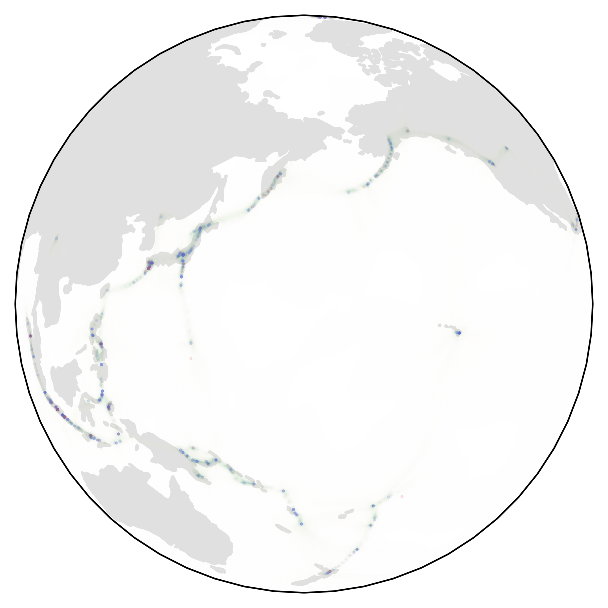
\includegraphics[width=\textwidth]{images/rsgm/pdf_volcanoe_310122.pdf}
		\caption{Volcano}
	\end{subfigure}
	\hfill
	\begin{subfigure}{0.22\textwidth}
		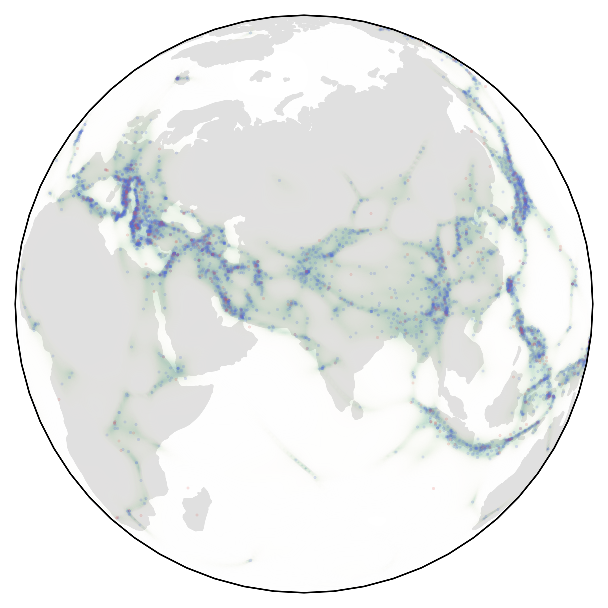
\includegraphics[width=\textwidth]{images/rsgm/pdf_earthquake_310122.pdf}
		\caption{Earthquake}
	\end{subfigure}
	\hfill
	\begin{subfigure}{0.22\textwidth}
		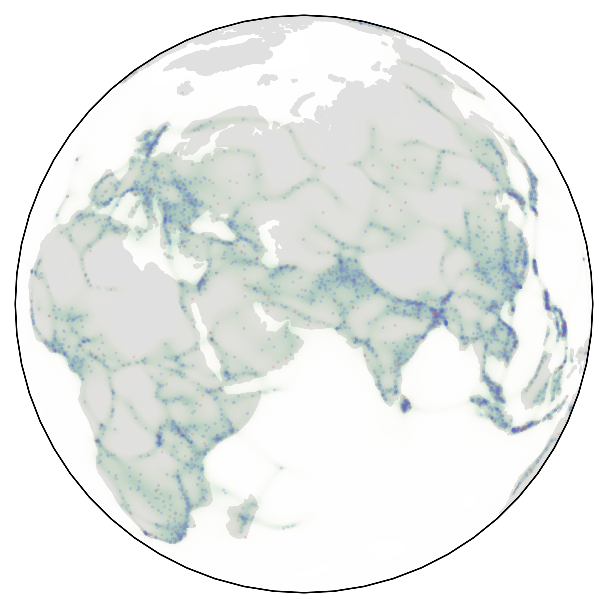
\includegraphics[width=\textwidth]{images/rsgm/pdf_flood_310122.pdf}
		\caption{Flood}
	\end{subfigure}
	\hfill
	\begin{subfigure}{0.22\textwidth}
		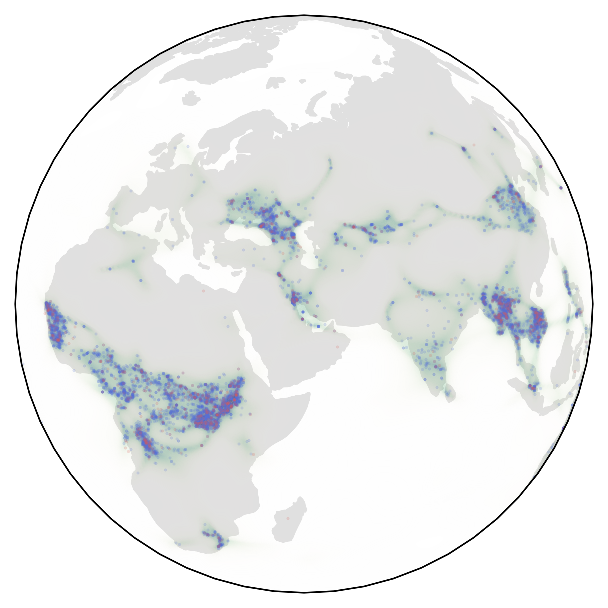
\includegraphics[width=\textwidth]{images/rsgm/pdf_fire_310122.pdf}
		\caption{Fire}
	\end{subfigure}
	\caption{
		Trained score-based generative models on earth sciences data.
		The learned density is colored green-blue.
		Blue and red dots represent training and testing datapoints, respectively.
	}
	\label{fig:geoscience}
\end{figure*}
\subsection{Synthetic data on tori}
\label{sec:exp_torus}
\begin{figure*}[t]
	\centering
	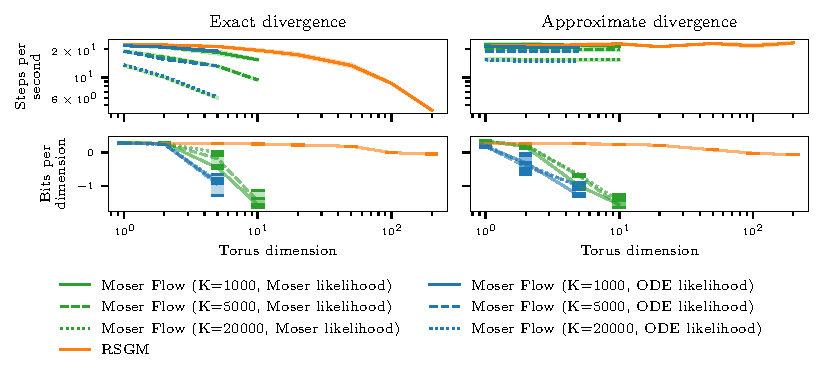
\includegraphics[width=\textwidth]{images/rsgm/high-dim.pdf}
	\caption{Comparison of Moser flows and RSGMs training speed and performance on the synthetic high-dimension torus task.
		Moser flows trained with \(\lambda_{\min}=1\).
		We report two likelihoods, the `Moser' closed form density---not guaranteed to be normalized---and the `ODE' likelihood given by solving an augmented ODE (as in CNFs) with the vector field induced by the Moser flow density---which is guaranteed to have unit volume.
	}
	\label{fig:high-dim}
\end{figure*}

We now move to another manifold, that is the torus \(\mathbb{T}^d = {\mathbb{S}^1 \times \dots \times \mathbb{S}^1}\), so as to assess the scalability of the different methods with respect to the dimension \(d\).
We consider a wrapped Gaussian target distribution on \(\mathbb{T}^d\) with a random mean and unit variance.
Moser flows'~\parencite{rozen2021moser} loss involves a regularization term which involves an integral over the manifold, approximated by a Monte Carlo (MC) estimator with uniform proposal.
This term regularizes Moser flows towards probability measures, i.e.\ with unit volume.
We thus expect Moser flows to fail in high-dimension as the number of samples \(K\) required for the MC estimator to be accurate will grows as \(\mathcal{O}(\mathrm{e}^d)\), and the memory required to compute this estimator grows either in \(\mathcal{O}(Kd)\) for exact divergences or \(\mathcal{O}(K)\) for approximated divergences (see \cref{tab:comparison_methods}).

In \Cref{fig:high-dim}, we observe that RSGMs are able to fit well the target distribution even in high dimension, with a linear or constant computational cost---depending on the divergence estimator.
In contrast, Moser flows scale poorly with the dimension, to the extent that we are unable to train them for \(d \ge 10\).
This is due to the combination of the complexity which grows linearly with both the dimension \(d\) and the number of MC samples \(K\), which itself ought to grow exponentially with \(d\)---as discussed in the previous paragraph.
This is illustrated by the gap between the `Moser' and `ODE' likelihoods which increases with the manifold dimension (see left \Cref{fig:high-dim}).

\subsection{Synthetic data on the Special Orthogonal group}
\label{sec:exp_so3}
In order to demonstrate the broad range of applicability of our model we now turn to the task of density estimation on the special orthogonal group \(\mathrm{SO}_d(\R) = \cbr{\mathrm{Q} \in \mathrm{M}_d(\R) \;:\;\mathrm{Q} \mathrm{Q}^\top = \m{I}, \ \det(\mathrm{Q})=1}\).
We consider the synthetic dataset consisting of samples in \(\mathrm{SO}_3(\R)\) from a mixture of wrapped normal distributions with \(M\) components.
We compare RSGMs against Moser flows and a wrapped-exponential baseline inspired by \textcite{falorsi2019reparameterizing}---where we parametrize a standard Euclidean SGM on \(\mathfrak{so}(3)\) that is then pushed-forward on \(\mathrm{SO}_3(\R)\).
RSGMs are trained using the \(\ell_{t|0}\) (DSM) loss with the Varadhan approximation (see \cref{tab:sm_losses}).
From \cref{tab:so3} we observe that, RSGMs perform consistently, whether the target distribution has few or many mixture components \(M\), as opposed to Exp-wrapped SGMs and Moser flows which only perform well in some range of \(M\).
Similarly to \cref{sec:exp_torus}, we find Moser flows to be much slower to train due to the large number of Monte Carlo samples needed in the reguralizer (\(K=10^4\)).
We also note from \cref{tab:so3} that the number of score network evaluations (NFE) is significantly lower for RSGMs, and is particularly detrimental for Moser flows (\(\gg 10^3\)).

\begin{figure*}[t]
	\centering
	\begin{subfigure}[t]{0.48\textwidth}
		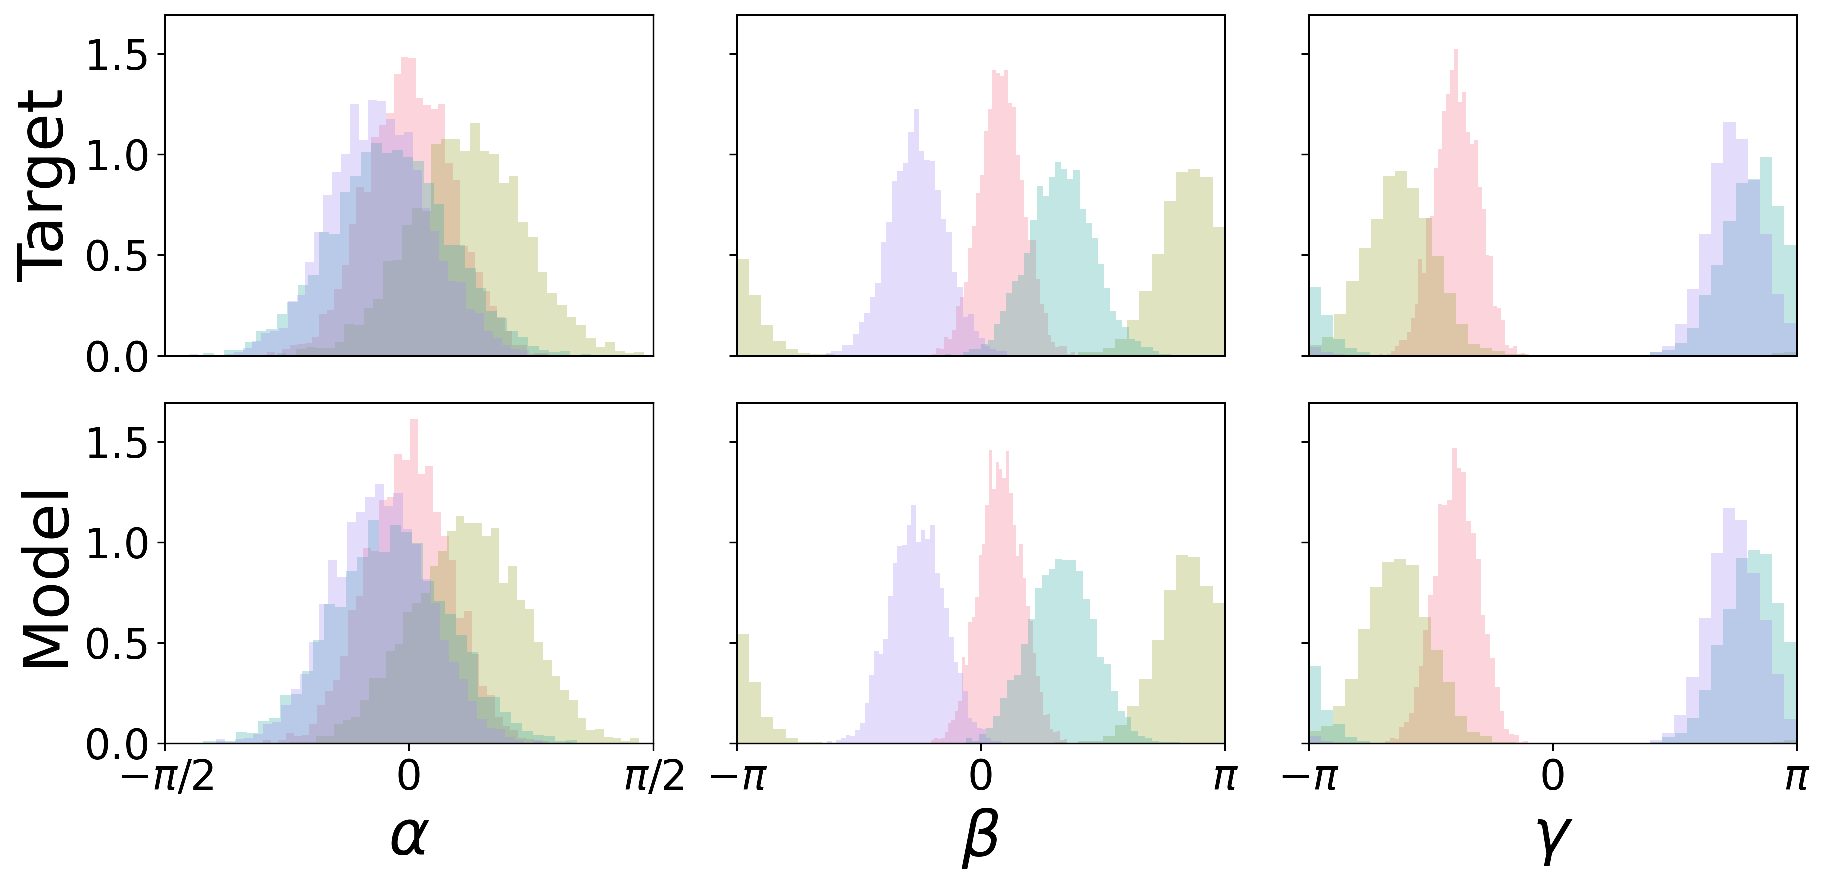
\includegraphics[width=\textwidth]{images/rsgm/so3_conditional.pdf}
		\caption{Histograms of \(\mathrm{SO}_3(\R)\) samples from a target mixture distribution with \(M=4\) components, represented via their Euler angles.}
		\label{fig:so3_conditional}
	\end{subfigure}
	\hfill
	\begin{subfigure}[t]{0.48\textwidth}
		
\includegraphics[width=\textwidth]{{images/rsgm/so3_heatmap}.pdf}
		\caption{
			RSGMs are much more robust to hyperparameters than Exp-wrapped SGMs.
			The diffusion coefficient is given by \(\sigma(t, \v{X}_t) = \sqrt{\beta(t)}\), \(\beta(t) = \beta_{0} + (\beta_{f} - \beta_{0})t\).
		}
		\label{fig:so3_heamtap}
	\end{subfigure}
	\caption{
		Trained score-based generative models on synthetic \(\mathrm{SO}_3(\R)\) data.
	}
	\label{fig:so3}
\end{figure*}
\begin{table*}[t]
	\centering
	\small
	\begin{tabular}{lrrrrrrrr}
		\toprule
		\multirow{2}{4.5em}{Method} & \multicolumn{2}{c}{\(M=16\)}                & \multicolumn{2}{c}{\(M=32\)}              & \multicolumn{2}{c}{\(M=64\)}                                                                                                                                                  \\ \cmidrule(lr){2-3} \cmidrule(lr){4-5} \cmidrule(lr){6-7}
		                            & log-likelihood                            & NFE                                     & log-likelihood                            & NFE                                      & log-likelihood                             & NFE                                     \\

		\midrule

		Moser Flow                  & \({0.85_{\pm 0.03}}\)                       & \({2.3_{\pm 0.5}}\)                       & \({0.17_{\pm 0.03}}\)                       & \({2.3_{\pm 0.9}}\)                        & \(\v{-0.49_{\pm 0.02}}\)                     & \({7.3_{\pm 1.4}}\)                       \\ Exp-wrapped SGM           & \cellcolor{blue!
		20} \(\v{0.87_{\pm 0.04}}\)   & \cellcolor{blue!20} \({0.5_{\pm 0.1}}\)     & \cellcolor{blue!20} \({0.16_{\pm 0.03}}\) & \cellcolor{blue!20} \({0.5_{\pm 0.0}}\)     & \cellcolor{blue!20} \({-0.58_{\pm 0.04}}\) & \cellcolor{blue!20} \({0.5_{\pm 0.0}}\)                                                \\
		RSGM                        & \cellcolor{blue!20} \(\v{0.89_{\pm 0.03}}\) & \cellcolor{blue!20} \(\v{0.1_{\pm 0.0}}\) & \cellcolor{blue!20} \(\v{0.20_{\pm 0.03}}\) & \cellcolor{blue!20} \(\v{0.1_{\pm 0.0}}\)  & \cellcolor{blue!20} \(\v{-0.49_{\pm 0.02}}\) & \cellcolor{blue!20} \(\v{0.1_{\pm 0.0}}\) \\

		\bottomrule
	\end{tabular}
	\caption{
		Test log-likelihood and associated number of function evaluations (NFE) in \(10^3\) on the synthetic mixture distribution with \(M\) components on \(\mathrm{SO}_3(\R)\).
		Bold indicates best results (up to statistical significance).
		Means and standard deviations are computed over 5 different runs.
		Novel methods are shown with blue shading.
	}
	\label{tab:so3}
\end{table*}

\subsection{Synthetic data on hyperbolic space}

Finally we demonstrate RSGM on a non-compact manifold: the two dimensional hyperbolic space \(\mathbb{H}^2\), which is defined as the simply connected space of constant negative curvature.
We use Langevin dynamics as the noising process (\cref{eq:langevin}) and target a wrapped Gaussian as the invariant distribution.
We again consider a synthetic dataset of samples from a mixture of exp-wrapped normal distribution.
From \cref{fig:hyperbolic}, we can qualitatively see that both score-based models are able to fit the target distribution.

\begin{figure}[t]
	\centering
	\hfill
	\begin{subfigure}[t]{0.28\textwidth}
		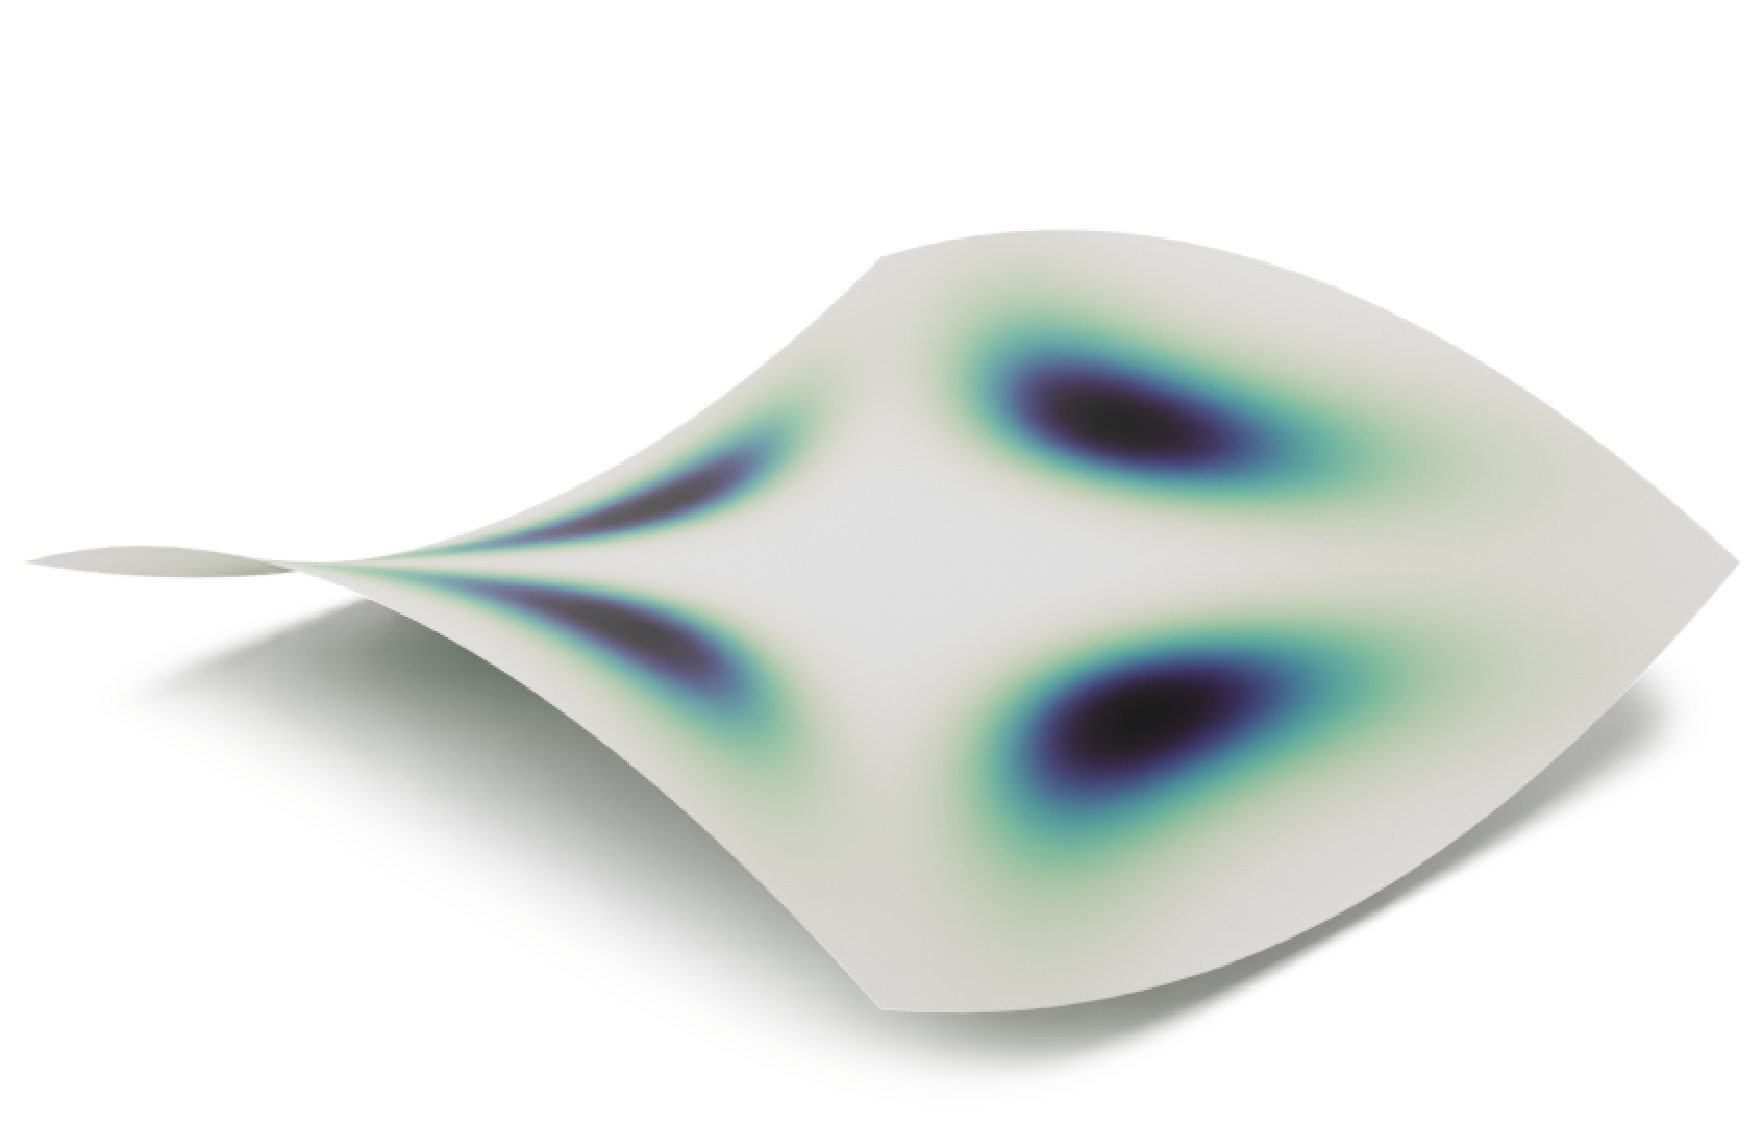
\includegraphics[width=\textwidth, trim={0.0em 0.0em 0.0em 5em},clip]{images/rsgm/hyperbolic/ref.pdf}
		\caption{Target distribution.}
	\end{subfigure}
	\hfill
	\begin{subfigure}[t]{0.28\textwidth}
		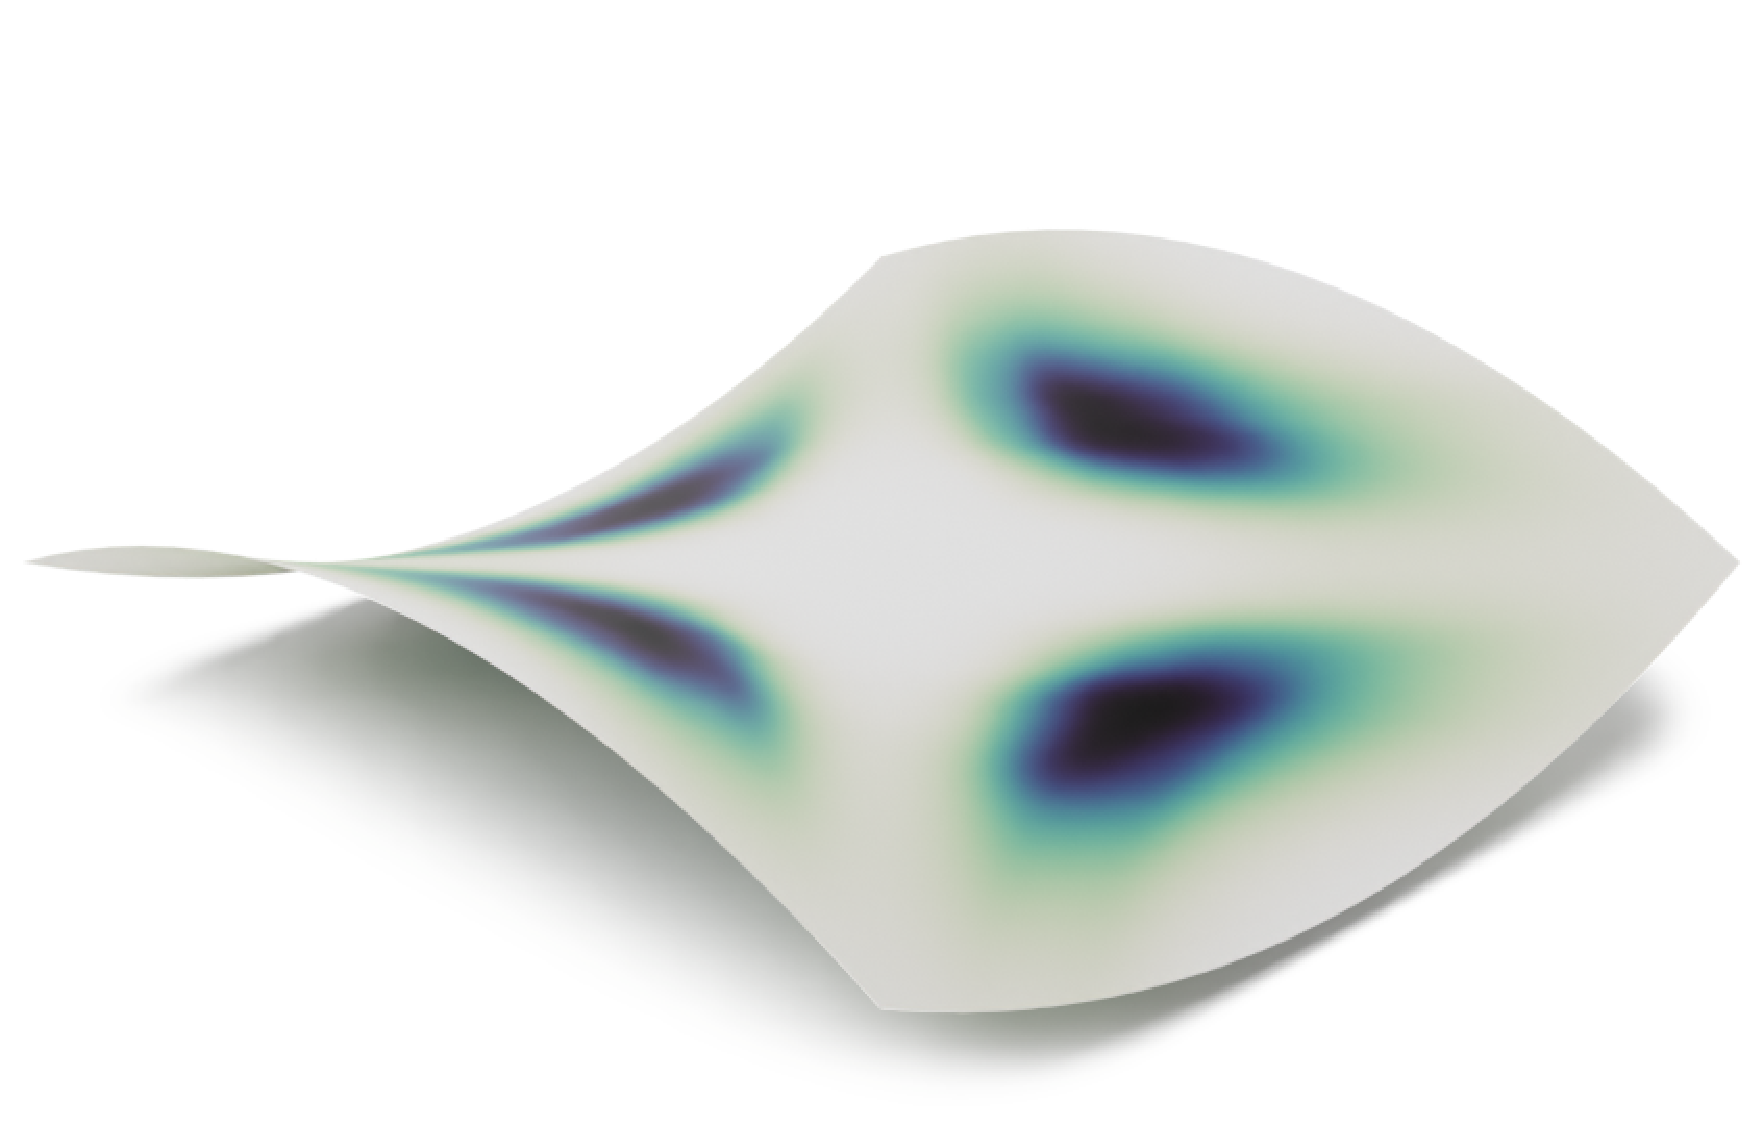
\includegraphics[width=\textwidth, trim={0.0em 0.0em 0.0em 5em},clip]{images/rsgm/hyperbolic/exp_wrap.pdf}
		\caption{Exp-wrapped SGM.}
	\end{subfigure}
	\hfill
	\begin{subfigure}[t]{0.28\textwidth}
		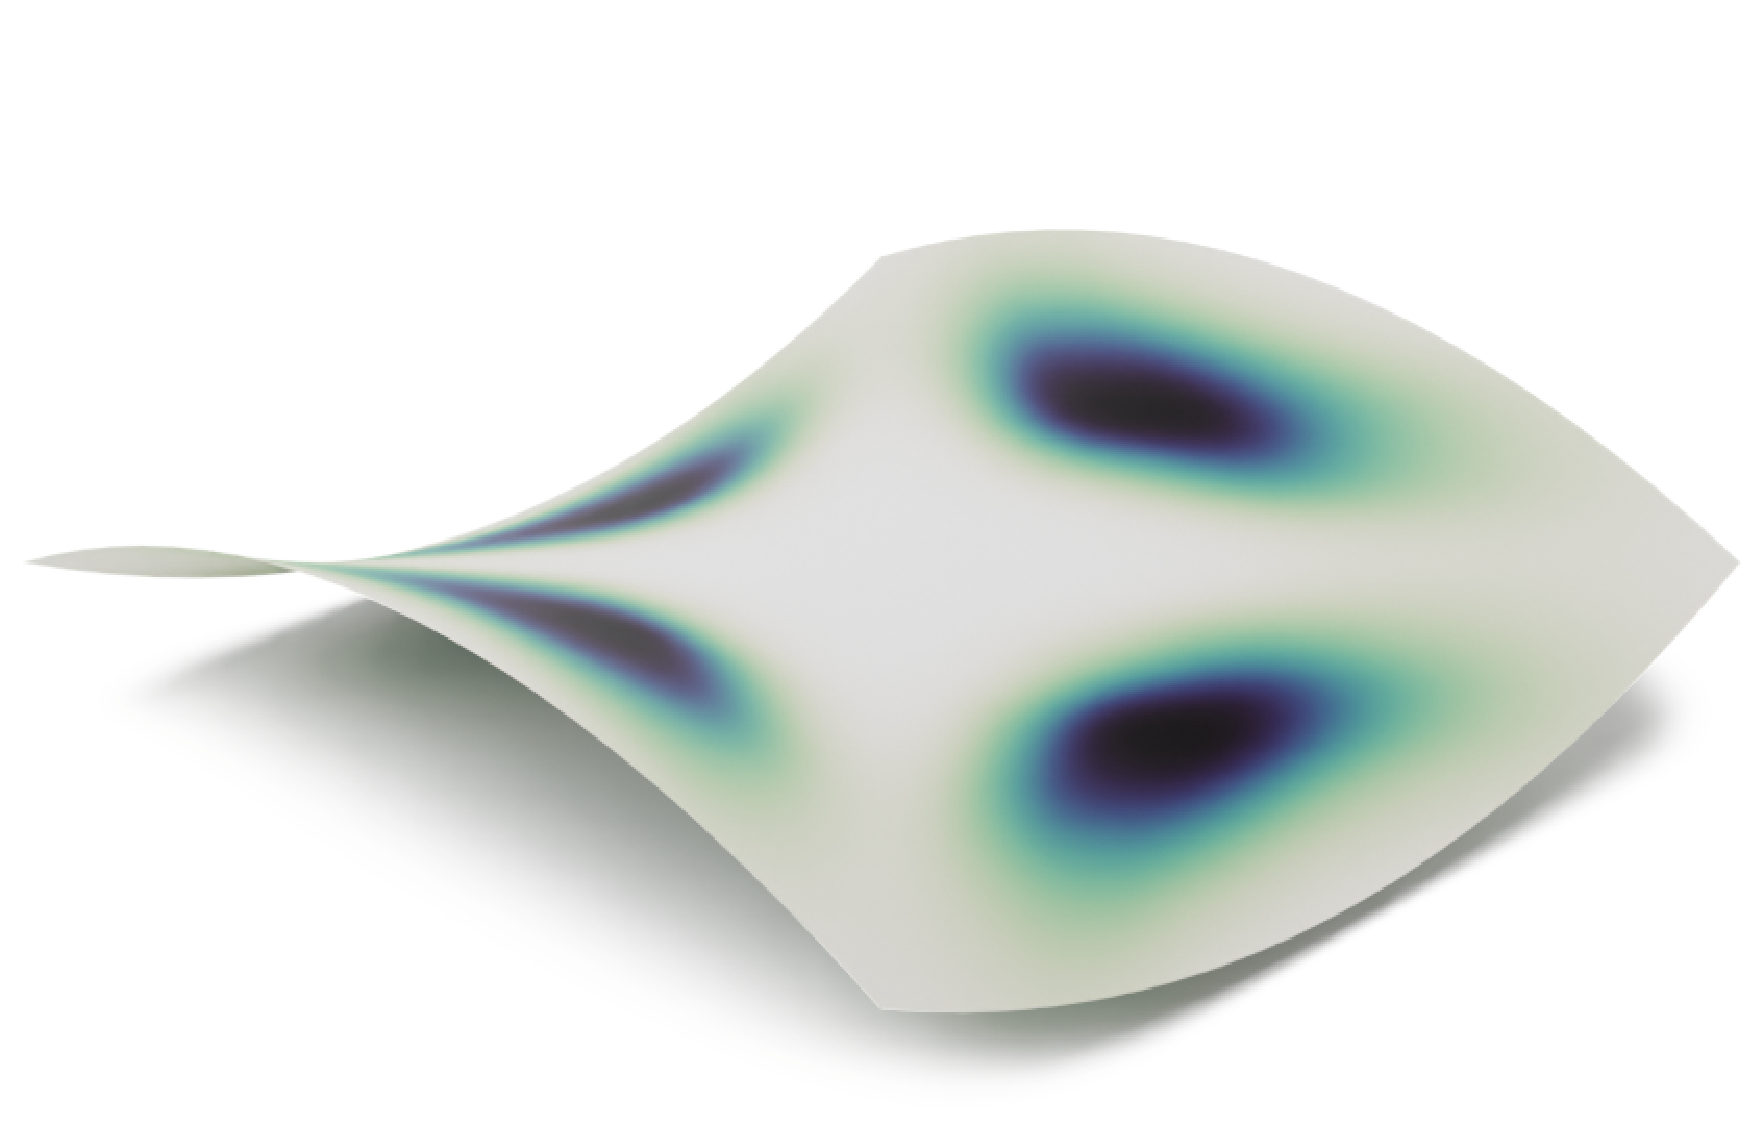
\includegraphics[width=\textwidth, trim={0.0em 0.0em 0.0em 5em},clip]{images/rsgm/hyperbolic/rsgm_quadratic.pdf}
		\caption{RSGM.}
	\end{subfigure}
	\hfill
	\caption{Samples from different probability distributions on \(\mathbb{H}^2\) coloured w.r.t\ their density.}
	\label{fig:hyperbolic}
\end{figure}

\section{Conclusion}
In this chapter we introduced Riemannian score-based generative models (RSGMs), a class of deep generative models that represent target densities supported on Riemannian manifolds, as the time-reversal of Langevin dynamics. 
The main benefits of our method stems from its scalability to high dimensions, its applicability to a broad class of manifolds due to the diversity of available loss functions, its robustness and crucially its capacity to model complex datasets while incoperating the geometry of the data.
We also provided theoretical guarantees on the convergence of these models. 
There is a large class of manifold that we cannot target with this method however, namely \emphhyperref{manifolds with boundary}{}.
The next chapter of this thesis focuses on this unresolved case.

\todo{mention Huang RDM}

% Another promising extension concerns stochastic control on manifolds and more precisely, deriving efficient algorithms to solve Schrödinger bridges (Thornton et al., 2022) in the same spirit as De Bortoli et al. (2021) on Euclidean state spaces